% Generated by Sphinx.
\documentclass[letterpaper,10pt,french]{manual}
\usepackage[utf8]{inputenc}
\usepackage[T1]{fontenc}
\usepackage{babel}
\usepackage{times}
\usepackage[Sonny]{fncychap}
\usepackage{longtable}
\usepackage{sphinx}


\title{openMairie - Guide du développeur Documentation}
\date{30 December 2010}
\release{0.0}
\author{openMairie}
\newcommand{\sphinxlogo}{}
\renewcommand{\releasename}{Version}
\makeindex
\makemodindex
\newcommand\PYGZat{@}
\newcommand\PYGZlb{[}
\newcommand\PYGZrb{]}
\newcommand\PYGaz[1]{\textcolor[rgb]{0.00,0.63,0.00}{#1}}
\newcommand\PYGax[1]{\textcolor[rgb]{0.84,0.33,0.22}{\textbf{#1}}}
\newcommand\PYGay[1]{\textcolor[rgb]{0.00,0.44,0.13}{\textbf{#1}}}
\newcommand\PYGar[1]{\textcolor[rgb]{0.73,0.38,0.84}{#1}}
\newcommand\PYGas[1]{\textcolor[rgb]{0.25,0.44,0.63}{\textit{#1}}}
\newcommand\PYGap[1]{\textcolor[rgb]{0.00,0.44,0.13}{\textbf{#1}}}
\newcommand\PYGaq[1]{\textcolor[rgb]{0.38,0.68,0.84}{#1}}
\newcommand\PYGav[1]{\textcolor[rgb]{0.00,0.44,0.13}{\textbf{#1}}}
\newcommand\PYGaw[1]{\textcolor[rgb]{0.13,0.50,0.31}{#1}}
\newcommand\PYGat[1]{\textcolor[rgb]{0.73,0.38,0.84}{#1}}
\newcommand\PYGau[1]{\textcolor[rgb]{0.32,0.47,0.09}{#1}}
\newcommand\PYGaj[1]{\textcolor[rgb]{0.00,0.44,0.13}{#1}}
\newcommand\PYGak[1]{\textcolor[rgb]{0.14,0.33,0.53}{#1}}
\newcommand\PYGah[1]{\textcolor[rgb]{0.00,0.13,0.44}{\textbf{#1}}}
\newcommand\PYGai[1]{\textcolor[rgb]{0.73,0.38,0.84}{#1}}
\newcommand\PYGan[1]{\textcolor[rgb]{0.13,0.50,0.31}{#1}}
\newcommand\PYGao[1]{\textcolor[rgb]{0.25,0.44,0.63}{\textbf{#1}}}
\newcommand\PYGal[1]{\textcolor[rgb]{0.00,0.44,0.13}{\textbf{#1}}}
\newcommand\PYGam[1]{\textbf{#1}}
\newcommand\PYGab[1]{\textit{#1}}
\newcommand\PYGac[1]{\textcolor[rgb]{0.25,0.44,0.63}{#1}}
\newcommand\PYGaa[1]{\textcolor[rgb]{0.19,0.19,0.19}{#1}}
\newcommand\PYGaf[1]{\textcolor[rgb]{0.25,0.50,0.56}{\textit{#1}}}
\newcommand\PYGag[1]{\textcolor[rgb]{0.13,0.50,0.31}{#1}}
\newcommand\PYGad[1]{\textcolor[rgb]{0.00,0.25,0.82}{#1}}
\newcommand\PYGae[1]{\textcolor[rgb]{0.13,0.50,0.31}{#1}}
\newcommand\PYGaZ[1]{\textcolor[rgb]{0.25,0.44,0.63}{#1}}
\newcommand\PYGbf[1]{\textcolor[rgb]{0.00,0.44,0.13}{#1}}
\newcommand\PYGaX[1]{\textcolor[rgb]{0.25,0.44,0.63}{#1}}
\newcommand\PYGaY[1]{\textcolor[rgb]{0.00,0.44,0.13}{#1}}
\newcommand\PYGbc[1]{\textcolor[rgb]{0.78,0.36,0.04}{#1}}
\newcommand\PYGbb[1]{\textcolor[rgb]{0.00,0.00,0.50}{\textbf{#1}}}
\newcommand\PYGba[1]{\textcolor[rgb]{0.02,0.16,0.45}{\textbf{#1}}}
\newcommand\PYGaR[1]{\textcolor[rgb]{0.25,0.44,0.63}{#1}}
\newcommand\PYGaS[1]{\textcolor[rgb]{0.13,0.50,0.31}{#1}}
\newcommand\PYGaP[1]{\textcolor[rgb]{0.05,0.52,0.71}{\textbf{#1}}}
\newcommand\PYGaQ[1]{\textcolor[rgb]{0.78,0.36,0.04}{\textbf{#1}}}
\newcommand\PYGaV[1]{\textcolor[rgb]{0.25,0.50,0.56}{\textit{#1}}}
\newcommand\PYGaW[1]{\textcolor[rgb]{0.05,0.52,0.71}{\textbf{#1}}}
\newcommand\PYGaT[1]{\textcolor[rgb]{0.73,0.38,0.84}{#1}}
\newcommand\PYGaU[1]{\textcolor[rgb]{0.13,0.50,0.31}{#1}}
\newcommand\PYGaJ[1]{\textcolor[rgb]{0.56,0.13,0.00}{#1}}
\newcommand\PYGaK[1]{\textcolor[rgb]{0.25,0.44,0.63}{#1}}
\newcommand\PYGaH[1]{\textcolor[rgb]{0.50,0.00,0.50}{\textbf{#1}}}
\newcommand\PYGaI[1]{\fcolorbox[rgb]{1.00,0.00,0.00}{1,1,1}{#1}}
\newcommand\PYGaN[1]{\textcolor[rgb]{0.73,0.73,0.73}{#1}}
\newcommand\PYGaO[1]{\textcolor[rgb]{0.00,0.44,0.13}{#1}}
\newcommand\PYGaL[1]{\textcolor[rgb]{0.02,0.16,0.49}{#1}}
\newcommand\PYGaM[1]{\colorbox[rgb]{1.00,0.94,0.94}{\textcolor[rgb]{0.25,0.50,0.56}{#1}}}
\newcommand\PYGaB[1]{\textcolor[rgb]{0.25,0.44,0.63}{#1}}
\newcommand\PYGaC[1]{\textcolor[rgb]{0.33,0.33,0.33}{\textbf{#1}}}
\newcommand\PYGaA[1]{\textcolor[rgb]{0.00,0.44,0.13}{#1}}
\newcommand\PYGaF[1]{\textcolor[rgb]{0.63,0.00,0.00}{#1}}
\newcommand\PYGaG[1]{\textcolor[rgb]{1.00,0.00,0.00}{#1}}
\newcommand\PYGaD[1]{\textcolor[rgb]{0.00,0.44,0.13}{\textbf{#1}}}
\newcommand\PYGaE[1]{\textcolor[rgb]{0.25,0.50,0.56}{\textit{#1}}}
\newcommand\PYGbg[1]{\textcolor[rgb]{0.44,0.63,0.82}{\textit{#1}}}
\newcommand\PYGbe[1]{\textcolor[rgb]{0.40,0.40,0.40}{#1}}
\newcommand\PYGbd[1]{\textcolor[rgb]{0.25,0.44,0.63}{#1}}
\newcommand\PYGbh[1]{\textcolor[rgb]{0.00,0.44,0.13}{\textbf{#1}}}
\begin{document}

\maketitle
\tableofcontents



Ce document a pour but de guider les développeurs dans la mise en oeuvre
d'un projet openMairie.

Avec plus de 30 applications développées pour les collectivités locales accessibles
sur le site \href{http://openmairie.org}{http://openmairie.org}, nous souhaitons au travers de ce guide , diffuser notre
expérience auprès  des collectivités et des acteurs économiques du libre qui les accompagnent.
Bonne lecture, et n'hésitez pas à nous faire part de vos remarques à l'adresse suivante :
\href{mailto:contact@openmairie.org}{contact@openmairie.org}

Si vous débutez, il est préférable de commencer par le chapître
``créer une application'' qui permet de prendre en main facilement le générateur et le
framework openMairie en vous guidant pas à pas dans le mise en place d'une
gestion de courrier.

Le chapître sur le ``framework'' complète l'exemple ci dessus en vous décrivant
le paramètrage, les classes formulaires et éditions du framework. Il a pour but
de vous informer de manière complète sur le fonctionnement du framework

Le chapître consacré au ``générateur'' décrit dans le détail le fonctionnement
de cet outil et de ses assistants.

Enfin ce document rassemble toutes les règles de codage du projet
openMairie, ainsi que des outils pour aider et guider les développeurs de la
communauté.

Les règles indiquées doivent être appliquées pour qu'un projet puisse
intégrer la distribution openMairie car l'objectif est de faciliter la
lisibilité et la maintenance du code ainsi que la prise en main par les
collectivités.

Cette création est mise à disposition selon le Contrat Paternité-Partage des
Conditions Initiales à l'Identique 2.0 France disponible en ligne
\href{http://creativecommons.org/licenses/by-sa/2.0/fr/}{http://creativecommons.org/licenses/by-sa/2.0/fr/} ou par courrier postal à
Creative Commons, 171 Second Street, Suite 300, San Francisco,
California 94105, USA.


\chapter{Créer une application}

\resetcurrentobjects
\hypertarget{--doc-utilisation/index}{}\hypertarget{index}{}
Ce chapitre vous propose de créer une application de gestion de courrier pas à pas.

\resetcurrentobjects
\hypertarget{--doc-utilisation/creer_base}{}

\hypertarget{creer-base}{}\section{Créer la base de données}

Vous devez au préalable copier openmairie\_exemple dans le repertoire www de votre serveur apache

Il vous est proposé de créer la base de données sous mysql :
\begin{itemize}
\item {} 
Créer une base de données appellée ``openmairie''

\item {} 
Créer les tables nécessaires au framework openMairie avec le fichier sql
\begin{quote}

data/mysql/init.sql
\end{quote}

\item {} 
Creer les tables necessaires a notre exemple
\begin{itemize}
\item {} 
table courrier

\begin{Verbatim}[commandchars=@\[\]]
courrier        int 8       cle primaire
dateenvoi       date
objetcourrier   text
emetteur        int8        cle secondaire
service         int8        cle secondaire
\end{Verbatim}

\item {} 
table emetteur

\begin{Verbatim}[commandchars=@\[\]]
emetteur        int 8       cle primaire
nom             varchar 20
prenom          varchar 20
\end{Verbatim}

\item {} 
table service

\begin{Verbatim}[commandchars=@\[\]]
service         int 8        cle primaire
libelle         varchar 20
\end{Verbatim}

\end{itemize}

\item {} 
modifier le paramétrage openMairie pour faire un accès à la base créée si votre base a un nom différent d'openMairie :
\begin{quote}

dyn/database.inc.php

voir framework/parametrage
\end{quote}

\item {} 
accéder avec votre navigateur sur openmairie\_exemple

\begin{Verbatim}[commandchars=@\[\]]
login : demo
mot de passe : demo
\end{Verbatim}

\end{itemize}

Le script mysql de création de la base de l'exemple est le suivant

\begin{Verbatim}[commandchars=@\[\]]
--
-- Structure de la table 'courrier'
--

CREATE TABLE courrier (
  courrier int(8) NOT NULL,
  dateenvoi date NOT NULL,
  objetcourrier text NOT NULL,
  emetteur int(8) NOT NULL,
  service int(8) NOT NULL,
  PRIMARY KEY  (courrier)
) TYPE=MyISAM;

--
-- Structure de la table 'emetteur'
--

CREATE TABLE emetteur (
  emetteur int(8) NOT NULL,
  nom varchar(20) NOT NULL,
  prenom varchar(20) NOT NULL,
  PRIMARY KEY  (emetteur)
) TYPE=MyISAM;

--
-- Structure de la table 'service'
--

CREATE TABLE service (
  service int(8) NOT NULL,
  libelle varchar(20) NOT NULL,
  PRIMARY KEY  (service)
) TYPE=MyISAM;
\end{Verbatim}

\resetcurrentobjects
\hypertarget{--doc-utilisation/utiliser_generateur}{}

\hypertarget{utiliser-generateur}{}\section{Créer les formulaires}

Nous allons maintenant créer les formulaires à l'aide du générateur

Pour cela, il faut aller dans le menu administration -\textgreater{} generateur

Vous devez avoir 3 nouveaux boutons : courrier, service, emetteur

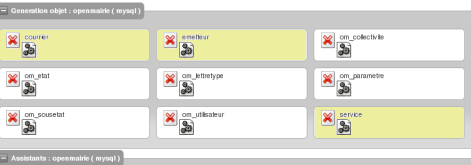
\includegraphics{utilisation_1.png}

Avant de commencer, l'utilisateur apache (www-data) doit avoir les droits
d'écriture dans les repertoires /gen , /sql et /obj


\subsection{Générer les formulaires et édition du courrier}

En appuyant sur le bouton de courrier, vous avez les choix de génération

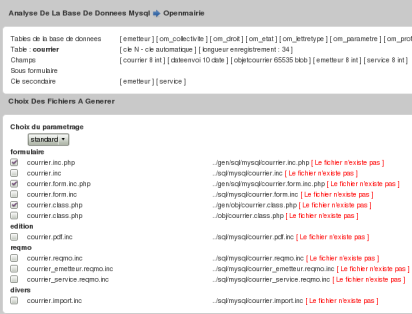
\includegraphics{utilisation_2.png}

Au préalable, le générateur fait une analyse de la base de données

\begin{Verbatim}[commandchars=@\[\]]
Tables de la base de donnees
            @PYGZlb[] emetteur @PYGZrb[] @PYGZlb[] service @PYGZrb[] et les tables om..

Table :
            courrier
            @PYGZlb[] cle N - cle automatique @PYGZrb[]
            @PYGZlb[] longueur enregistrement : 34 @PYGZrb[]

Champs
            @PYGZlb[] courrier 8 int @PYGZrb[]
            @PYGZlb[] dateenvoi 10 date @PYGZrb[]
            @PYGZlb[] objetcourrier 65535 blob @PYGZrb[]
            @PYGZlb[] emetteur 8 int @PYGZrb[]
            @PYGZlb[] service 8 int @PYGZrb[]
Sous formulaire
Cle secondaire
            @PYGZlb[] emetteur @PYGZrb[] @PYGZlb[] service @PYGZrb[]
\end{Verbatim}

Le générateur a détecté 2 clés secondaires et aucun sous formulaire

C'est pour cela qu'il propose 3 ``reqmo'' : 1 ``reqmo'' global et 2 ``reqmos'' suivant la clé secondaire

Par défaut, 3 options sont cochées, ce sont les 3 fichiers fabriqués par le générateur

Cochez toutes les options

\begin{Verbatim}[commandchars=@\[\]]
formulaire
    courrier.inc.php                ../gen/sql/mysql/courrier.inc.php
    courrier.inc                    ../sql/mysql/courrier.inc
    courrier.form.inc.php           ../gen/sql/mysql/courrier.form.inc.php
    courrier.form.inc               ../sql/mysql/courrier.form.inc
    courrier.class.php              ../gen/obj/courrier.class.php
    courrier.class.php              ../obj/courrier.class.php
edition
    courrier.pdf.inc                ../sql/mysql/courrier.pdf.inc
reqmo
    courrier.reqmo.inc              ../sql/mysql/courrier.reqmo.inc
    courrier@_emetteur.reqmo.inc ../sql/mysql/courrier@_emetteur.reqmo.inc
    courrier@_service.reqmo.inc      ../sql/mysql/courrier@_service.reqmo.inc
divers
    courrier.import.inc         ../sql/mysql/courrier.import.inc
\end{Verbatim}

En cliquant sur valider, vous avez le message

\begin{Verbatim}[commandchars=@\[\]]
Parametrage utilise : standard

* ecriture fichier ../gen/sql/mysql/courrier.inc.php
* ecriture fichier ../sql/mysql/courrier.inc
* ecriture fichier ../gen/sql/mysql/courrier.form.inc.php
* ecriture fichier ../sql/mysql/courrier.form.inc
* ecriture fichier ../gen/obj/courrier.class.php
* ecriture fichier ../obj/courrier.class.php
-@textgreater[]affichage colone ok 8,23529411765 @textgreater[]= 2.5
* ecriture fichier ../sql/mysql/courrier.pdf.inc
* ecriture fichier ../sql/mysql/courrier.reqmo.inc
* ecriture fichier ../sql/mysql/courrier@_emetteur.reqmo.inc
* ecriture fichier ../sql/mysql/courrier@_service.reqmo.inc
* ecriture fichier ../sql/mysql/courrier.import.inc
\end{Verbatim}

Le paramétrage utilisé est le paramétrage standard.

Vous pouvez le modifier : \emph{voir generateur/parametrage}

L'affichage par colone est ``ok'', ce qui veut dire que la taille des colones
dans le fichier pdf sera complet. (attention le script ne prend pas le champ blob)


\subsection{Générer les formulaires et édition de l'emetteur}

Nous allons procéder de la même manière avec le bouton emetteur.

L'analyse de la base de données est la suivante

\begin{Verbatim}[commandchars=@\[\]]
Tables de la base de donnees
                @PYGZlb[] courrier @PYGZrb[] @PYGZlb[] service @PYGZrb[] et les tables om ...

Table :
                emetteur
                @PYGZlb[] cle N - cle automatique @PYGZrb[]
                @PYGZlb[] longueur enregistrement : 48 @PYGZrb[]

Champs
                @PYGZlb[] emetteur 8 int @PYGZrb[]
                @PYGZlb[] nom 20 string @PYGZrb[]
                @PYGZlb[] prenom 20 string @PYGZrb[]

Sous formulaire
                @PYGZlb[] courrier @PYGZrb[]

Cle secondaire
\end{Verbatim}

Le générateur repère un sous formulaire courrier.
Effectivement, il y a une relation de un à plusieurs entre emetteur et courrier :
un emetteur peut avoir 0 à plusieurs courriers

En cliquant sur toutes les options, vous avez le message suivant

\begin{Verbatim}[commandchars=@\[\]]
Parametrage utilise : standard

* ecriture fichier ../gen/sql/mysql/emetteur.inc.php
* ecriture fichier ../sql/mysql/emetteur.inc
* ecriture fichier ../gen/sql/mysql/emetteur.form.inc.php
* ecriture fichier ../sql/mysql/emetteur.form.inc
* ecriture fichier ../gen/obj/emetteur.class.php
* ecriture fichier ../obj/emetteur.class.php
-@textgreater[]affichage colone ok 5,83333333333 @textgreater[]= 2.5
* ecriture fichier ../sql/mysql/emetteur.pdf.inc
* ecriture fichier ../sql/mysql/emetteur.reqmo.inc
* ecriture fichier ../sql/mysql/emetteur.import.inc
\end{Verbatim}


\subsection{Générer les formulaires et édition de service}

Nous allons procéder de la même manière avec le bouton service

L'analyse de la base de données est la suivante

\begin{Verbatim}[commandchars=@\[\]]
Tables de la base de donnees
            @PYGZlb[] courrier @PYGZrb[] @PYGZlb[] emetteur @PYGZrb[] et les tables om ..

Table :
        service
        @PYGZlb[] cle N - cle automatique @PYGZrb[] @PYGZlb[] longueur enregistrement : 28 @PYGZrb[]

Champs
        @PYGZlb[] service 8 int @PYGZrb[]
        @PYGZlb[] libelle 20 string @PYGZrb[]

Sous formulaire
        @PYGZlb[] courrier @PYGZrb[]

Cle secondaire
\end{Verbatim}

Le générateur repère un sous formulaire courrier.
Effectivement, il y a une relation de un à plusieurs entre service et courrier :
un service peut avoir 0 à plusieurs courriers

En cliquant sur toutes les options, vous avez le message suivant

\begin{Verbatim}[commandchars=@\[\]]
Parametrage utilise : standard

* ecriture fichier ../gen/sql/mysql/service.inc.php
* ecriture fichier ../sql/mysql/service.inc
* ecriture fichier ../gen/sql/mysql/service.form.inc.php
* ecriture fichier ../sql/mysql/service.form.inc
* ecriture fichier ../gen/obj/service.class.php
* ecriture fichier ../obj/service.class.php
-@textgreater[]affichage colone ok 10 @textgreater[]= 2.5
* ecriture fichier ../sql/mysql/service.pdf.inc
* ecriture fichier ../sql/mysql/service.reqmo.inc
* ecriture fichier ../sql/mysql/service.import.inc
\end{Verbatim}


\subsection{Integrer les formulaires dans le menu}

Pour accéder à nos formulaires, nous allons les intégrer dans le menu
( voir \emph{framework/parametrage/menu gauche})

Nous allons appeller le formulaire depuis le menu :

option application -\textgreater{} tab.php?obj=courrier

option parametrage -\textgreater{} tab.php?obj=emetteur

option parametrage -\textgreater{} tab.php?obj=service

Il faut ouvrir avec un éditeur le fichier dyn/menu.inc.php et insérer le code suivant

\begin{Verbatim}[commandchars=@\[\]]
       // *** APPLICATION ***
       // inserez ici les tables de votre application
         array@_push(@$links,
           array(
               "href" =@textgreater[] "../scr/tab.php?obj=courrier",
               "class" =@textgreater[] "courrier",
               "title" =@textgreater[] @_("courrier"),
               "right" =@textgreater[] "courrier"
           ));



   // *** TABLES DE PARAMETRAGE ***
   // inserer ici vos tables de parametres

     array@_push(@$links,
       array(
           "href" =@textgreater[] "../scr/tab.php?obj=emetteur",
           "class" =@textgreater[] "emetteur",
           "title" =@textgreater[] @_("emetteur"),
           "right" =@textgreater[] "emetteur"
       ));

       array@_push(@$links,
       array(
           "href" =@textgreater[] "../scr/tab.php?obj=service",
           "class" =@textgreater[] "service",
           "title" =@textgreater[] @_("service"),
           "right" =@textgreater[] "service"
       ));


Vous pouvez accéder à vos formulaires par le menu avec les options :
\end{Verbatim}

\textbf{application -\textgreater{} courrier}

Cette opération affiche la table courrier :

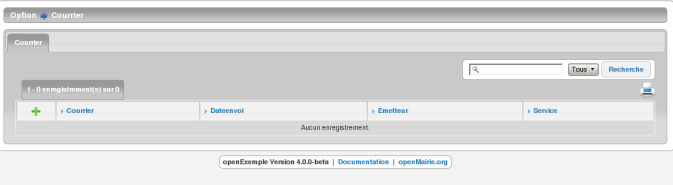
\includegraphics{utilisation_3.png}

On accéde en appuyant sur + au formulaire d'insertion ou les champs sont :
\begin{itemize}
\item {} 
la date du courrier avec calendrier

\item {} 
l'objet du courrier dans un champ textarea

\item {} 
deux controles ``select'' pour le service et l emetteur

\end{itemize}
\begin{quote}

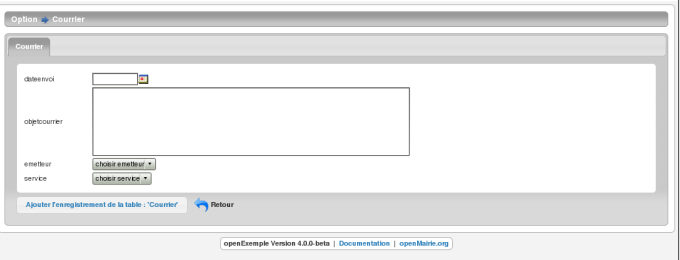
\includegraphics{utilisation_4.png}
\end{quote}

\textbf{parametrage -\textgreater{} emetteur}

Cette operation affiche la table emetteur :

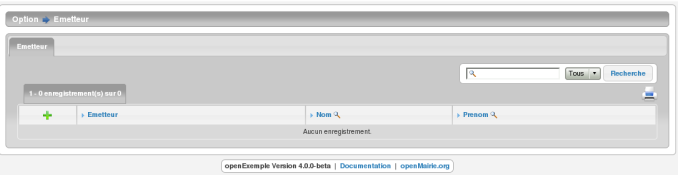
\includegraphics{utilisation_5.png}

En appuyant sur +, on accède à la saisie

L'onglet courrier est inactif tant que l'emetteur n est pas saisi et validé

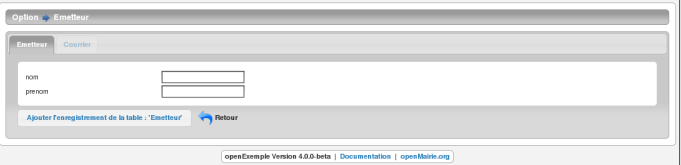
\includegraphics{utilisation_6.png}

\textbf{parametrage -\textgreater{} service}

Cette opération affiche la table service :

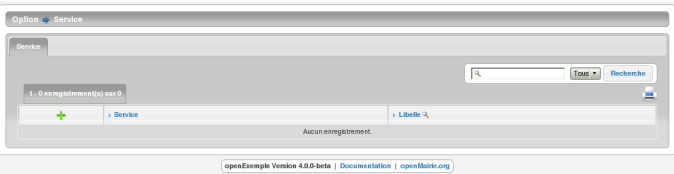
\includegraphics{utilisation_7.png}

En appuyant sur +, on accede à la saisie

L'onglet courrier est inactif tant que le service n est pas saisi

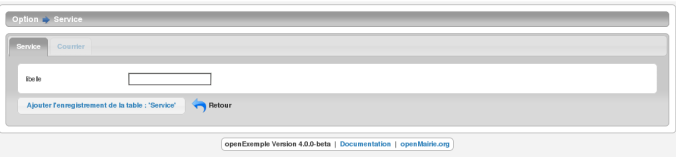
\includegraphics{utilisation_8.png}

Vous pouvez accéder aux éditions et requêtes mémorisées :

\textbf{export -\textgreater{} edition}

Cet option affiche l'ensemble des éditions pdf :

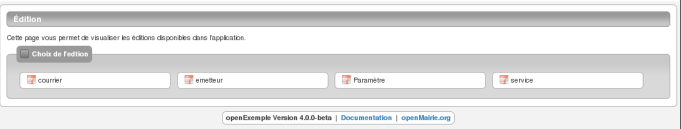
\includegraphics{utilisation_9.png}

pour en savoir plus voir \emph{framework/edition}

\textbf{export -\textgreater{} reqmo}

Cette option affiche les requêtes mémorisées :

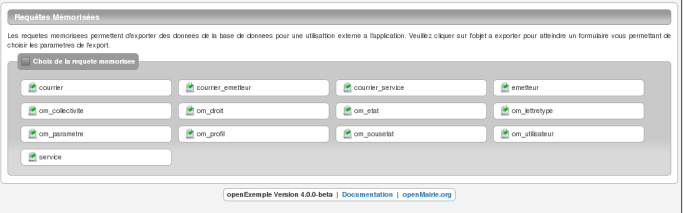
\includegraphics{utilisation_10.png}

pour en savoir plus voir \emph{framework/reqmo}

Vous pouvez accéder aux éditions en appuyant dans le formulaire d'affichage sur l'imprimante

Vous pouvez accéder au fichiers d'import

\textbf{administration -\textgreater{} import}

Cette option affiche les scripts d'imports :

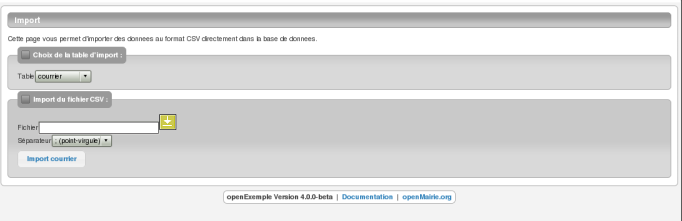
\includegraphics{utilisation_11.png}

pour en savoir plus voir \emph{framework/import}

\resetcurrentobjects
\hypertarget{--doc-utilisation/personnaliser}{}

\hypertarget{personnaliser}{}\section{Personnaliser son application}

Nous allons maintenant personnaliser notre application

Pour se faire, nous allons saisir le jeu de données suivantes

Vous pouvez le faire avec les formulaires, la création des tables stockant les
sequences est fait par le framework (methode setId des objets metier)  sinon vous pouvez exécuter
le script sql suivant

\begin{Verbatim}[commandchars=@\[\]]
-- insertion de deux emetteurs

INSERT INTO emetteur (emetteur, nom, prenom) VALUES
(1, 'dupont', 'pierre'),
(2, 'durant', 'jacques');

--
-- Structure de la table 'emetteur@_seq'
--

CREATE TABLE emetteur@_seq (
  id int(10) unsigned NOT NULL auto@_increment,
  PRIMARY KEY  (id)
) TYPE=MyISAM ;

--
-- Contenu de la table 'emetteur@_seq'
--

INSERT INTO emetteur@_seq (id) VALUES (2);

--
-- Contenu de la table 'service'
--

INSERT INTO service (service, libelle) VALUES
(1, 'informatique'),
(2, 'telephonie');


--
-- Structure de la table 'service@_seq'
--

CREATE TABLE service@_seq (
  id int(10) unsigned NOT NULL auto@_increment,
  PRIMARY KEY  (id)
) TYPE=MyISAM ;

--
-- Contenu de la table 'service@_seq'
--

INSERT INTO service@_seq (id) VALUES (2);

--
-- Contenu de la table 'courrier'
--

INSERT INTO courrier (courrier, dateenvoi, objetcourrier, emetteur, service) VALUES
(1, '2010-12-01', 'Proposition de fourniture de service', 1, 1),
(2, '2010-12-02', 'Envoi de devis pour formation openMairie', 2, 1);

--
-- Structure de la table 'service@_seq'
--

CREATE TABLE service@_seq (
  id int(10) unsigned NOT NULL auto@_increment,
  PRIMARY KEY  (id)
) TYPE=MyISAM ;

--
-- Contenu de la table 'service@_seq'
--

INSERT INTO service@_seq (id) VALUES (2);
\end{Verbatim}


\subsection{Faire un affichage courrier plus convivial}

L'affichage des courriers se fait avec les clés secondaires et non
les libellés.

Nous souhaitons avoir le nom et le prénom de l'emetteur et le libellé du service.

Dans le fichier sql/mysql/courrier.inc nous allons modifier les variables  \$table
et  \$champAffiche de la manière suivante (après la ligne include):

\begin{Verbatim}[commandchars=@\[\]]
@$table = DB@_PREFIXE."courrier  inner join ".DB@_PREFIXE."emetteur
                on emetteur.emetteur=courrier.emetteur
                inner join ".DB@_PREFIXE."service
                on service.service=courrier.service";

@$champAffiche=array('courrier',
                'concat(substring(dateenvoi,9,2),\'/\',substring(dateenvoi,6,2),
                                \'/\',substring(dateenvoi,1,4)) as dateenvoi',
                'concat(emetteur.nom,\' \',emetteur.prenom) as emetteur',
                'service.libelle as service');
\end{Verbatim}

Le résultat est le suivant

\begin{Verbatim}[commandchars=@\[\]]
Courrier Dateenvoi  Emetteur            Service
    1       01/12/2010      dupont pierre   informatique
    2       02/12/2010      durant jacques  informatique
\end{Verbatim}

De la même manière nous souhaitons rechercher dans les courriers sur le
nom de l'emetteur et sur le libellé du service. Dans le fichier sql/mysql/courrier.inc,
nous allons modifier la variable tableau \$champRecherche de la manière suivante

\begin{Verbatim}[commandchars=@\[\]]
@$champRecherche=array("emetteur.nom", "service.libelle");
\end{Verbatim}

Vous devez avoir dans la zone recherche la possibilité de selectionner

\begin{Verbatim}[commandchars=@\[\]]
Tous
emetteur@PYGbe[.]nom
service@PYGbe[.]libelle
\end{Verbatim}

Nous souhaitons maintenant avoir les derniers courriers au début de la page affichée et nous
pouvons le faire en insérant la variable \$tri dans courrier.inc de la manière suivante:

\begin{Verbatim}[commandchars=@\[\]]
@$tri= " order by dateenvoi desc";
\end{Verbatim}

Le résultat est le suivant

\begin{Verbatim}[commandchars=@\[\]]
2       02/12/2010      durant jacques          informatique
1       01/12/2010          dupont pierre           informatique
\end{Verbatim}

\emph{Pour en savoir plus sur ces variables voir framework/affichage}


\subsection{Rendre obligatoire des champs}

Nous avons affiché le courrier avec une jointure de type ``inner''.
Donc s'il n'y a pas de lien sur le service et/ou l'emetteur, l'enregistrement
n'apparaitra pas. Il faut rendre obligatoire la saisie de  l'emetteur et du service (auquel le courrier est affecté)

Nous allons surcharger la méthode verifier() dans obj/courrier.class.php de la manière suivante
(par défaut le premier champ, ici dateenvoi est obligatoire, cet option est modifiable
dans le générateur)

La methode à insérer apres le constructeur est la suivante

\begin{Verbatim}[commandchars=@\[\]]
function verifier(@$val,@&@$db,@$DEBUG) {
    parent::verifier(@$val,@$db,@$DEBUG);
    @$f="@&nbsp!@&nbsp;@&nbsp;@&nbsp;@&nbsp;";
    @$imgv="@textless[]img src='../img/punaise.png' style='vertical-align:middle' hspace='2' border='0'@textgreater[]";
    if (@$this-@textgreater[]valF@PYGZlb[]'service'@PYGZrb[]==""){
        @$this-@textgreater[]msg= @$this-@textgreater[]msg.@$imgv.@_('service')."@&nbsp;".@_('obligatoire').@$f;
        @$this-@textgreater[]correct=False;
    }
    if (@$this-@textgreater[]valF@PYGZlb[]'emetteur'@PYGZrb[]==""){
        @$this-@textgreater[]msg= @$this-@textgreater[]msg.@$imgv.@_('emetteur')."@&nbsp;".@_('obligatoire').@$f;
        @$this-@textgreater[]correct=False;
    }
}
\end{Verbatim}

La commande ``parent::verifier(\$val,\$db,\$DEBUG);'' permet de ne pas neutraliser la
fonction surchargée (ici dans gen/obj/courrier.class.php)

\emph{Pour plus d'information voir le châpitre framework/methode}


\subsection{Valoriser un champ par défaut}

Pour simplifier la saisie, nous souhaitons mettre la date du jour dans le
champ dateenvoi n ajout de courrier.

Nous allons surcharger la methode setVal() dans obj/courrier.class.php
de la manière suivante

\begin{Verbatim}[commandchars=@\[\]]
function setVal(@&@$form, @$maj, @$validation, @&@$db, @$DEBUG=null){
    parent::setVal(@$form, @$maj, @$validation, @$db, @$DEBUG=null);
    if (@$validation==0) {
        if (@$maj == 0){
            @$form-@textgreater[]setVal("dateenvoi", date('Y-m-d'));
        }
    }
}
\end{Verbatim}

Le champ dateenvoi contient la date systeme (date(`Y\_m-d')) si la validation est égal à 0
et si \$maj est égal à 0 (ajout).


\subsection{Mettre en majuscule un champ}

Nous souhaitons maintenant mettre en majuscule le champ ``nom'' de la table emetteur.
Nous allons surcharger la methode setOnchange() dans
obj/emetteur.class.php de la manière suivante

\begin{Verbatim}[commandchars=@\[\]]
function setOnchange(@&@$form,@$maj){
    parent::setOnchange(@$form,@$maj);
    @$form-@textgreater[]setOnchange("nom","this.value=this.value.toUpperCase()");
}
\end{Verbatim}

A la saisie ou à la modification du nom, le champ se met en majuscule.


\subsection{Principe à retenir}

Voila quelques exemples des possibilités de modification dans les fichiers sql
(repertoire sql/ ....) et dans les methodes de l'objet (repertoire obj/ ...)

En aucun cas, il ne faut modifier les fichiers dans gen/ qui est l'espace de travail du générateur,
\textbf{Nous allons dans le prochain chapître modifier la base et  regénérer les écrans sans mettre en danger
votre personnalisation.}

\resetcurrentobjects
\hypertarget{--doc-utilisation/modifier_base}{}

\hypertarget{modifier-base}{}\section{Modifier la base et re générer}

Le framework openMairie permet de modifier la base , et de prendre en
compte ces modifications en regénérant les scripts sans mettre en péril
la personnalisation que vous avez effectuée

Nous vous proposons de rajouter un champ registre dans la table courrier
et de rajouter l'adresse dans la table emetteur.


\subsection{Rajouter un champ registre dans courrier}

Il est proposer de rajouter un champ registre dans le courrier dont le but
est de stocker le numéro de registre du courrier sous la forme annee\_numero\_d\_ordre

Nous allons d'abord créer un champ registre dans courrier de la manière suivante

\begin{Verbatim}[commandchars=@\[\]]
ALTER TABLE courrier ADD registre VARCHAR( 20 ) NOT NULL ;
\end{Verbatim}

Vous devez regénérer votre application courrier dans l'option du menu : administration -\textgreater{} generateur -\textgreater{} courrier
et laisser cochées les options par défaut :
\begin{quote}

gen/obj/courrier.class.php

gen/sql/mysql/courrier.inc.php

gen/sql/mysql/courrier.form.inc.php
\end{quote}

Validez l'opération.

Vous pouvez remarquer si vous allez sur le formulaire un nouveau champ registre
en fin de formulaire. Votre personnalisation n'est pas affectée.

Nous voulons que le numero de registre se mette en ajout de manière automatique ,
une fois le formulaire validé:

Il faut donc surcharger les méthodes suivantes dans obj/courrier.class.php

\begin{Verbatim}[commandchars=@\[\]]
// pour que registre ne soit pas modifiable
function setType(@&@$form,@$maj) {
    parent::setType(@&@$form,@$maj);
     @$form-@textgreater[]setType('registre', 'hiddenstatic');
}


// pour la mise a jour de la séquence avant l ajout de l enregistrement

function triggerajouter(@$id,@&@$db,@$val,@$DEBUG)
{
    //  prochain numero de registre
    //  fonction DB pear
    @$temp= @$db-@textgreater[]nextId("registre");
    // fabrication du numero annee@_no@_d@_ordre
    @$temp= date('Y')."-".@$temp;
    @$this-@textgreater[]valF@PYGZlb[]'registre'@PYGZrb[] = @$temp;
}
\end{Verbatim}

Si vous souhaitez que registre apparaisse dans l'affichage de la table, vous
devez aussi modifier le tableau champAffiche de sql/mysql/courrier.inc de la manière
suivante

\begin{Verbatim}[commandchars=@\[\]]
@$champAffiche=array('courrier',
    'concat(substring(dateenvoi,9,2),\'/\',substring(dateenvoi,6,2),\'/\',substring(dateenvoi,1,4)) as dateenvoi',
    'concat(emetteur.nom,\' \',emetteur.prenom) as emetteur',
    'service.libelle as service',
    'registre');
\end{Verbatim}

Votre affichage de la table courrier est modifié.


\subsection{Rajouter l'adresse dans emetteur}

Il est proposé de rajouter l'adresse de l'emetteur à savoir : le libellé, le code postal et
la ville. Le script sql est le suivant

\begin{Verbatim}[commandchars=@\[\]]
ALTER TABLE emetteur ADD adresse VARCHAR( 40 ) NOT NULL ,
ADD cp VARCHAR( 5 ) NOT NULL ,
ADD ville VARCHAR( 40 ) NOT NULL ;
\end{Verbatim}

Vous devez regénérer votre application courrier en allant dans l'option du menu :
administration -\textgreater{} generateur -\textgreater{} emetteur et laisser cochées les options par défaut :
\begin{quote}

gen/obj/emetteur.class.php

gen/sql/mysql/emetteur.inc.php

gen/sql/mysql/emetteur.form.inc.php
\end{quote}

Validez l'opération.

N'ayant pas modifié sql/mysql/emetteur.inc, le framework fonctionne avec le code généré


\subsection{Améliorer la présentation du formulaire emetteur}

Nous pouvons continuer à améliorer les présentations de nos formulaires
en utilisant les méthodes setGroupe() et setRegroupe() dans le script
obj/emetteur.class.php

Il vous est proposé d'insérer dans votre script obj/emetteur.class.php
le code suivant

\begin{Verbatim}[commandchars=@\[\]]
function setGroupe(@&@$form, @$maj) {
    @$form-@textgreater[]setGroupe('nom','D');
    @$form-@textgreater[]setGroupe('prenom','F');

    @$form-@textgreater[]setGroupe('cp','D');
    @$form-@textgreater[]setGroupe('ville','F');
}

function setRegroupe(@&@$form,@$maj){
    @$form-@textgreater[]setRegroupe('nom','D', @_('nom'), "collapsible");
    @$form-@textgreater[]setRegroupe('prenom','F','');

    @$form-@textgreater[]setRegroupe('adresse','D', ('adresse'), "startClosed");
    @$form-@textgreater[]setRegroupe('cp','G','');
    @$form-@textgreater[]setRegroupe('ville','F','');
}
\end{Verbatim}

Le fieldset nom est affiché par défaut, pas celui de l'adresse.

Vos formulaires sont maintenant au point.

Le paragraphe suivant vous indique les surcharges d'openCourrier que vous
pouvez intégrer dans votre exemple, maintenant que vous avez la a méthode.


\subsection{Les surcharges d'openCourrier}

Vous pouvez utiliser openCourrier version 3.0.0 qui est téléchargeable au lien suivant :

\href{http://adullact.net/frs/?group\_id=297}{http://adullact.net/frs/?group\_id=297}

La base de données d'openCourrier est plus complexe. C'est ainsi que
courrier a deux sous formulaires : tache et dossier et qu'il
est aussi possible de compléter l'objet du courrier avec une bible.

Si les surcharges qui ont été faites dans notre exemple sont celles d'openCourrier, il y a
d'autre surcharge dans le script courrier.class.php d'openCourrier,  :

Les méthodes setLib, setGroupe et setRegroupe permettent \textbf{une présentation
en fieldset}  du courrier (utilisation des champs vide1 à 5 voir sql/mysql/courrier.form.inc)

\textbf{La gestion des emetteurs enregistre dans la table courrier l'emetteur} (voir la méthode
setType qui utilise les combos, la méthode setSelect qui les paramétre
et la méthode triggerAjouterapres qui enregistre l'emetteur saisi en formulaire courrier
dans la table emetteur si la case vide5 est cochée)

Il est possible d'\textbf{afficher un courrier préalablement scanné} et d'
\textbf{enregistrer le fichier pdf dans dossier.class.php} après avoir écrit dessus
le numéro de registre (Voir les méthodes setType et triggerAjouterapres).

Il y a d'autres objet métier qui ont des surcharges intéressantes :

Dans dossier.class.php, vous avez un exemple de type upload pour télécharger des
fichiers.

L'objet obj/tachenonsolde.class.php est un \textbf{exemple de surcharge de tache.class.php}
qui affiche que les tâches non soldées

openCourrier fonctionne avec des restrictions d'accès par service et \textbf{les
méthodes de login} ont été modifiées dans obj/utils.class.php ainsi qu'
utilisateur.class.php qui a dans openCourrier un champ service.

Vous pouvez aussi regarder \textbf{deux scripts de traitement} :
\begin{itemize}
\item {} 
trt/num\_registre.php qui remet à 0 le numéro de registre

\item {} 
trt/archivage.php qui tranfere en archive les courriers avant une date

\end{itemize}

Vous avez plus de détail sur les traitements dans le chapître
\emph{framework/util} notament sur la mise à jour du registre.

\resetcurrentobjects
\hypertarget{--doc-utilisation/utiliser_assistant}{}

\hypertarget{utiliser-assistant}{}\section{Créer ses états}

Il vous est proposé de créer un état des courriers par service

Il sera utilisé dans ce chapître l'assistant état et sous état du générateur


\subsection{Créer l'état service}

Nous allons utiliser l'assistant état du générateur dans le menu :

administration -\textgreater{} générateur  : assistant

Choisir ``créer un état''

Puis choisr dans le select, l'option service

Ensuite avec la touche ``ctrl'', sélectionner les champs service et libellé

Appuyer ensuite sur ``import service dans la base''

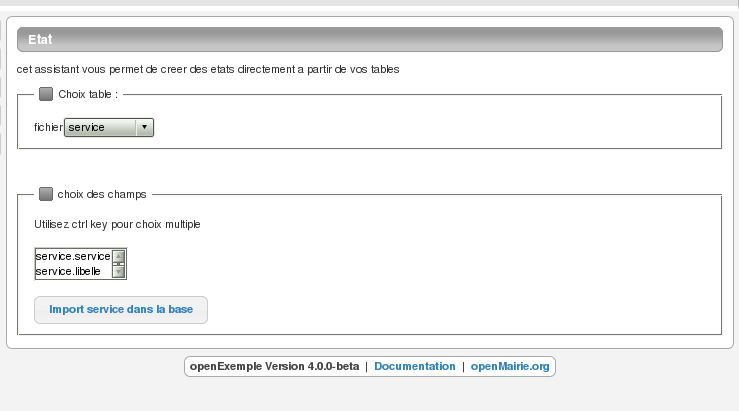
\includegraphics{utilisation_12.png}

Un message apparait ``service enregistré''

Vous avez créé un enregistrement qui a pour identifiant ``service'' dans
la table ``om\_etat''.

Il faut maintenant permettre l'accès dans l'affichage du service.

Ouvrer le fichier sql/mysql/service.inc

Ajouter le script suivant

\begin{Verbatim}[commandchars=@\[\]]
@$href@PYGZlb[]3@PYGZrb[] = array(
    "lien" =@textgreater[] "../pdf/pdfetat.php?obj=".@$obj."@&amp;idx=",
    "id" =@textgreater[] "",
    "lib" =@textgreater[] "@textless[]img src=\"../img/pdf-16x16.png\" alt=\""
             .@_("Edition PDF")."\" title=\"".@_("Edition PDF")."\" /@textgreater[]",
);
\end{Verbatim}

Nous rajoutons la ligne 3 dans le tableau href. Vous avez un état lié
à l'affichage du service.

Il y a des exemples d'utilisation de href dans om\_collectivité, om\_etat,
om\_utilisateur ...


\subsection{Créer le sous état courrier}

Nous allons utiliser l'assistant sous état du générateur dans le menu :

administration -\textgreater{} générateur  : assistant : sousetat

Nous choisissons la table courrier et nous surlignons les champs
dateenvoi, registre, objetcourrier et emetteur

Nous choisissons courrier.service comme clé secondaire pour faire le lien
avec service.

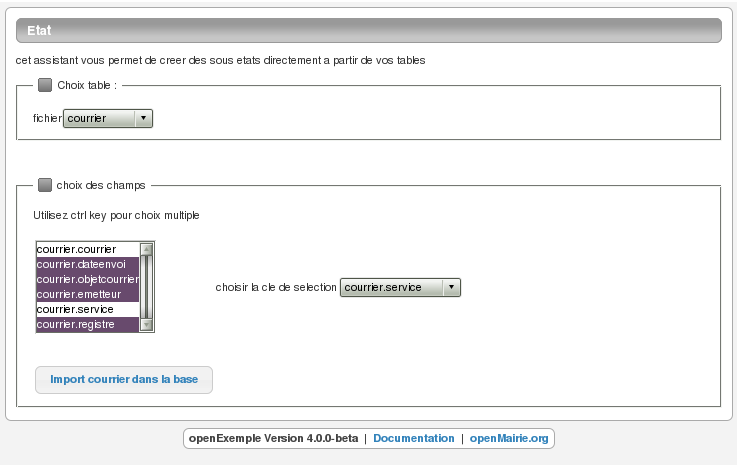
\includegraphics{utilisation_13.png}

En cliquant sur ``import courrier dans la base'', vous créez un enregistrement
ayant pour identifiant ``courrier.service'' dans la table om\_sousetat


\subsection{Associer le sous état ``courrier'' à l'état ``service''}

Vous devez rendre d'abord votre sous etat courrier.service actif pour pouvoir l'associer.

Allez dans l option du menu : administration -\textgreater{} sous etat

Recherchez le sous état ``courrier.service'' et modifier le en cochant sur actif
(1er fieldset)

Il vous faut maintenant associer le sous état ``courrier.service'' à l'état ``service''

Allez dans l'option du menu administration -\textgreater{} etat.

Cherchez l'état ``courrier'' et modifiez le dans le fieldset (à déplier)
sous état selection, choisissez le sous état ``courrier.service''

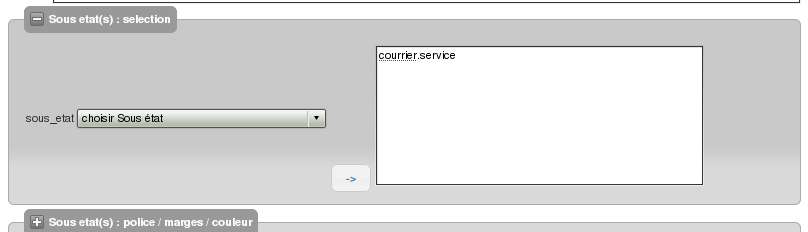
\includegraphics{utilisation_14.png}

Vous avez désormais un état des courriers par service :

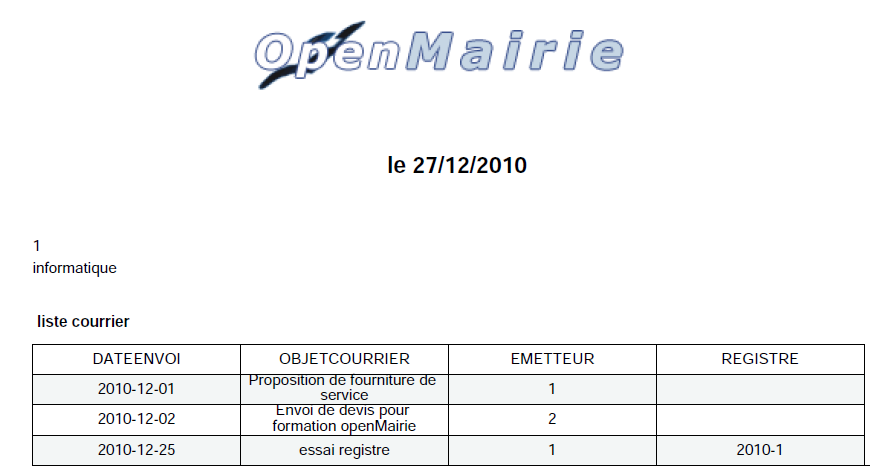
\includegraphics{utilisation_15.png}


\subsection{Mettre le nom et le prénom de l'emetteur dans le sous état}

Nous souhaitons mettre le nom et le prénom de l'emetteur à la place de
la clé secondaire.

Vous devez modifier la requête sql de l'enregistrement courrier.service
dans la table om\_sousetat de la manière suivante

\begin{Verbatim}[commandchars=@\[\]]
select  courrier.dateenvoi as dateenvoi,
        courrier.objetcourrier as objetcourrier,
        concat(emetteur.nom,' ',emetteur.prenom) as emetteur,
        courrier.registre as registre
        from @&DB@_PREFIXEcourrier inner join @&DB@_PREFIXEemetteur
        on emetteur.emetteur = courrier.emetteur
        where courrier.service='@&idx'
\end{Verbatim}

Votre nouvel état a la forme suivante :

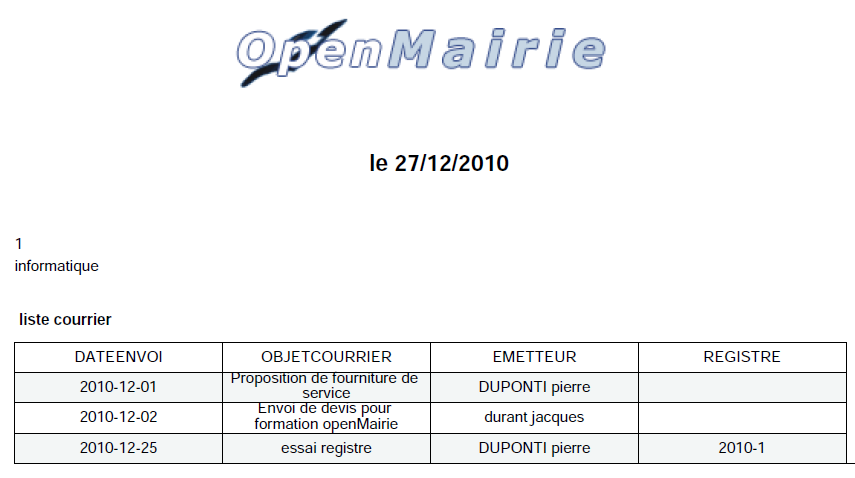
\includegraphics{utilisation_16.png}

Vous avez de nombreux exemples d'utilisation d'état et de sous état dans
les applications openMairie.

Une utilisation originale a été faite pour le cerfa du recensement dans
openRecensement où à la place du logo, il a été mis une image du cerfa.

On ne peut cependant pas faire tous les états et il est fort possible que vous ayez des
etats spécifiques. Vous avez des exemples d'utilisation spécifique des méthodes
de fpdf dans openElec : carte électorale, liste électorale ...

Vous pouvez compléter votre information avec le chapître \emph{framework/edition}
et regarder les possibilités de paramétrage du générateur \emph{generateur/parametrage}
pour la réalisation d'état customisé.


\chapter{Le framework}

\resetcurrentobjects
\hypertarget{--doc-framework/index}{}
openMairie\_exemple est le framework de base dans lequel vous pouvez
développer votre propre application.

openMairie\_exemple est \textbf{téléchargeable sur le site de l'adullact}

\href{http://adullact.net/frs/?group\_id=329}{http://adullact.net/frs/?group\_id=329}

Il est proposé ici de décrire le fonctionnement du framework.

Dans un environnement LAMP/WAMP, le framework integre des composants au travers
de classes qui permettent de créer des formulaires et des états.
Ces classes sont surchargées par les objets métier à créer.

openMairie integre de nombreux composants : DBPEAR et FPDF dans toutes les applications,
mais aussi ARTISHOW (pour les graphes), NSOAP pour les web services,
JQUERY pour l'ergonomie, OPENLAYERS pour l interface SIG ...

DBPEAR est un abstracteur de base de données qui permet d'utiliser diverses bases de données notament MYSQL ou POSTGRESQL.

FPDF est le composant qui permet de gérer le PDF.

Le développement consiste à créer des objets métier  qui surchargent la classe abstraite
dbformdyn.class.php (composant openMairie). De base, les données de la base de données sont récupérés pour le
formulaire (longueur, max, nom).
\begin{itemize}
\item {} 
dbformdyn.class.php ; assure la liaison entre le formulaire et la base de données

\item {} 
formulairedyn.class.php : rassemble toutes les méthodes permettant de construire des formulaires

\begin{Verbatim}[commandchars=@\[\]]
Ce chapître propose de vous décrire les outils de base du framework de la manière suivante :

    - le paramétrage général du framework
    - la gestion des accès du framework et la multi collectivite
    - les méthodes pour construire des formulaires avec le framework
    - les outils d'édition du framework
    - l'outil de requête paramétrable du framework
    - l'ergonomie intégrant jquery
    - la gestion de traitement et la construction de programme spécifiques avec les utilitaires
    - l'import des données CSV du framework
    - l'interface geographique intégrant openlayers avec openCimetiere
    - l'envoi de mail intégrant phpmail avec openPersonnalite (en projet)
    - le fonctionnement d'artichow dans openResultat (en projet)
    - le fonctionnement du nusoap dans openFoncier (enprojet)
    - l'utilisation de fpdf pour écrire dans un pdf dans openCourrier (en projet)
    - la mise en oeuvre d'un éditeur wysiwyg pour l'édition des états (en projet)
\end{Verbatim}

\end{itemize}

\resetcurrentobjects
\hypertarget{--doc-framework/parametrage}{}

\hypertarget{parametrage}{}\section{Paramétrage du framework}

Le paramétrage de l application se fait dans le répertoire /dyn.

Il est proposé dans ce chapitre de décrire les différents fichiers de paramétrage.

Les fichiers de paramétrage sont les suivants

\begin{Verbatim}[commandchars=@\[\]]
dyn/database.inc.php           connexion a la base de données
dyn/menu.inc.php               menu principal à gauche
dyn/action.inc                 menu haut
dyn/shortslink.inc             lien sous menu haut
dyn/tbd.inc                    tableau de bord
dyn/locales.inc                application
dyn/config.inc.php             application
dyn/include.inc.php            chemin d'accès aux librairies
dyn/debug.inc.php              mode debug
dyn/version.inc                paramétrage de la version

README.txt                     fichiers textes
HISTORY.txt
SPECIFIC.txt
LICENCE.txt
TODO.txt
INSTALL.txt
\end{Verbatim}


\subsection{La connexion de la base de donnees}

Le paramétrage de la connexion se fait dans : \emph{dyn/database.inc.php}

Le paramétrage par défaut est dans le tableau \$conn{[}1{]} pour la base 1 :

Il peut être paramétré plusieurs bases : conn{[}1{]} , conn{[}2{]} ...

conn{[}1{]} est un tableau php qui contient les parametres de connexion suivants

\begin{Verbatim}[commandchars=@\[\]]
'titre          =@textgreater[] 'openxxx',       @PYGZlb[]parametrage openmairie@PYGZrb[]
'phptype'       =@textgreater[] 'mysql',         mysql ou 'pgsql' @PYGZlb[]parametrage dbpear@PYGZrb[]
'dbsyntax'      =@textgreater[] '',              @PYGZlb[]ne pas changer parametrage dbpear@PYGZrb[]
'username'      =@textgreater[] 'root',          @PYGZlb[]par defaut sur wamp easyphp ou lamp /
                                    a voir avec le fournisseur d acces le cas echeant@PYGZrb[]
'password'      =@textgreater[] ''               @PYGZlb[]par defaut sur wamp easyphp ou lamp /
                                    a voir avec le fournisseur d acces le cas echeant@PYGZrb[]
'protocol'      =@textgreater[] '',
'hostspec'      =@textgreater[] 'localhost',     @PYGZlb[]nom de serveur par defaut wamp ou easyphp@PYGZrb[]
'port'          =@textgreater[] '',              @PYGZlb[]ne pas changer parametrage dbpear@PYGZrb[]
'socket'        =@textgreater[] '',              @PYGZlb[]ne pas changer parametrage dbpear@PYGZrb[]
'nom de la base'=@textgreater[] 'openxxx',       @PYGZlb[]parametrage openmairie@PYGZrb[]
'format date'   =@textgreater[]'AAAA-MM-JJ'      @PYGZlb[]parametrage openmairie ne pas changer@PYGZrb[]
'shema'         =@textgreater[] ''               ou 'public' pour postgre
'prefixe'       =@textgreater[] ''
\end{Verbatim}

Il est possible de définir tout phptype : mysql, pgsql (postgresql), oci8 pour oracle.

Il faut voir la documentation de DB PEAR qui est le module d'abstraction utilisé
dans openMairie (version 4.0.0)


\subsection{Le menu principal}

Le paramétrage du menu se fait dans le fichier \emph{dyn/menu.inc.php}.

De base, les rubriques suivantes sont paramétrées dans le framework:

\begin{Verbatim}[commandchars=@\[\]]
application             vide par défaut, contient l'accès à votre application
export                  contient le script "edition" qui reprend
                            les éditions pdf des tables
                        contient le menu "reqmo" qui reprend les requêtes
                            mémorisées
traitement              vide par défaut, cet option contient les scripts de
                            traitement
parametrage             Cette option contient vos tables de paramétrage
administration          Les scripts de cet option contiennent tout les scripts
                            du framework pour le paramètrage de la collectivité,
                            des états / sous états  et la gestion des accès
\end{Verbatim}

Le paramétrage du menu se fait dans \$menu.

\$menu est le tableau associatif qui contient tout le menu de l'application,
il contient lui meme un tableau par rubrique, puis chaque
rubrique contient un tableau par lien :

Les caracteristiques de ce tableau sont les suivantes :
\begin{quote}

tableau rubrik

\begin{Verbatim}[commandchars=@\[\]]
title (obligatoire)
description (texte qui s'affiche au survol de la rubrique)
href (contenu du lien href)
class (classe css qui s'affiche sur la rubrique)
right (droit que l'utilisateur doit avoir pour visionner cette rubrique)
links (obligatoire)
\end{Verbatim}

tableau links

\begin{Verbatim}[commandchars=@\[\]]
title (obligatoire)
href (obligatoire) (contenu du lien href)
class (classe css qui s'affiche sur l'element)
right (droit que l'utilisateur doit avoir pour visionner cet element)
target (pour ouvrir le lien dans une nouvelle fenetre)
\end{Verbatim}
\end{quote}


\subsection{Le menu haut}

Le paramétrage du menu haut se fait dans le fichier \emph{dyn/action.inc.php}

Par défaut, il est paramétré le changement de mot de poste et la déconnexion

\$actions est le tableau associatif qui contient tous les liens présents dans
les actions à côté du login et du nom de la collectivite

les caractéristiques du tableau link sont les suivantes :

tableau link

\begin{Verbatim}[commandchars=@\[\]]
title (obligatoire)
description (texte qui s'affiche au survol de l'element)
href (obligatoire) (contenu du lien href)
class (classe css qui s'affiche sur l'element)
right (droit que l'utilisateur doit avoir pour visionner cet element)
target (pour ouvrir le lien dans une nouvelle fenetre)
\end{Verbatim}

Les liens sous le menu des actions se paramétrent dans le fichier : \emph{dyn/shortlinks.inc.php}

\$shortlinks est le tableau associatif qui contient tous les liens présents
dans les raccourcis qui se situent en dessous des actions du menu haut

Par défaut, il est paramétré l'accès au tableau de bord.

Les caracteristiques du tableau \$link sont les suivantes :

tableau link

\begin{Verbatim}[commandchars=@\[\]]
title @PYGZlb[]obligatoire@PYGZrb[]
description (texte qui s'affiche au survol de l'element)
href @PYGZlb[]obligatoire@PYGZrb[] (contenu du lien href)
class (classe css qui s'affiche sur l'element)
right (droit que l'utilisateur doit avoir pour visionner cet element)
target (pour ouvrir le lien dans une nouvelle fenetre)
\end{Verbatim}


\subsection{Le tableau de bord}

Le tableau de bord se paramètre dans le fichier \emph{dyn/tdb.inc}.

Le parametrage est libre et depend de l'application.

Ce fichier est appellé par le script scr/dashboard.php.

Nous proposons cet exemple de code

\begin{Verbatim}[commandchars=@\[\]]
@$description = @_("Bienvenue ").@$@_SESSION@PYGZlb[]"login"@PYGZrb[]."@textless[]br@textgreater[]";
@$f-@textgreater[]displayDescription(@$description);
\end{Verbatim}

Ce paramétrage va afficher ``bienvenue demo'' dans la page d'accueil ou
tableau de bord pour l'utilisateur ``demo''


\subsection{Les variables locales et la langue}

Les variables locales sont paramétrées dans le fichier \emph{dyn/locales.inc.php}

Ce fichier contient :
\begin{itemize}
\item {} 
le paramétrage du codage des caracteres

\begin{Verbatim}[commandchars=@\[\]]
define(@PYGaB[']@PYGaB[CHARSET]@PYGaB['], @PYGaB[']@PYGaB[ISO-8859-1]@PYGaB[']);
\end{Verbatim}

\item {} 
le dossier ou sont installées les variables du systeme

\begin{Verbatim}[commandchars=@\[\]]
define(@PYGaB[']@PYGaB[LOCALE]@PYGaB['], @PYGaB[']@PYGaB[fr@_FR]@PYGaB[']);
\end{Verbatim}

\item {} 
Le dossier contenant les locales et les fichiers de traduction

\begin{Verbatim}[commandchars=@\[\]]
define(@PYGaB[']@PYGaB[LOCALES@_DIRECTORY]@PYGaB['], @PYGaB[']@PYGaB[../locales]@PYGaB[']);
\end{Verbatim}

\item {} 
Le domaine de traduction

\begin{Verbatim}[commandchars=@\[\]]
define(@PYGaB[']@PYGaB[DOMAIN]@PYGaB['], @PYGaB[']@PYGaB[openmairie]@PYGaB[']);
\end{Verbatim}

\end{itemize}

Les zones à traduire sont sous le format : \_(``zone a traduire'')

Voir le chapître sur les outils : \emph{poEdit}


\subsection{Le paramétrage de l application metier}

L'application métier est paramétrée dans \emph{dyn/var.inc}

Ce script contient les paramétres globaux de l application .
Attention les paramètres s'appliquent à toutes les bases de l'application.

Le paramétrage spécifique par collectivité doit se faire dans la table om\_parametre

La configuration générale de l'application se fait aussi dans \emph{dyn/config.inc.php}.

Les paramètres sont récupérés avec la création d'un objet utils par :
\$f-\textgreater{}config{[}'nom\_du\_parametre'{]}

\emph{Voir framework/utilitaire}

Exemple de paramétrage avec openCourrier

\begin{Verbatim}[commandchars=@\[\]]
@$config@PYGZlb[]'application'@PYGZrb[] = @_("openCourrier");
@$config@PYGZlb[]'title'@PYGZrb[] = ":: ".@_("openMairie")." :: ".@_("openCourrier");
@$config@PYGZlb[]'session@_name'@PYGZrb[] = "openCourrier";
\end{Verbatim}
\begin{itemize}
\item {} 
le mode demonstration de l'application se paramétre avec \$config{[}'demo'{]}

\end{itemize}

Ce mode permet de pre-remplir le formulaire de login avec l'identifiant `demo' et le mot de passe `demo'

\begin{Verbatim}[commandchars=@\[\]]
@$config@PYGZlb[]'demo'@PYGZrb[] = false;  l'application n'est pas en mode démo
                  true; l'application est en mode démo

Attention, pour empêcher de changer le mot de passe, il faut paramétrer l'accès
dans la table om@_droit : password
\end{Verbatim}
\begin{itemize}
\item {} 
La configuration des extensions autorisees dans le module upload.php

\end{itemize}
\begin{quote}

Pour changer votre configuration, décommenter la ligne et modifier les extensions avec des ``;'' comme séparateur

\begin{Verbatim}[commandchars=@\[\]]
@$config@PYGZlb[]'upload@_extension'@PYGZrb[] = ".gif;.jpg;.jpeg;.png;.txt;.pdf;.csv;"
\end{Verbatim}
\end{quote}
\begin{itemize}
\item {} 
Le thème de l'application - les différents choix possibles se trouvent dans le

dossier : ../lib/jquery-ui/css/

Par defaut, le thème d'openExemple est ``om\_overcast''

\begin{Verbatim}[commandchars=@\[\]]
@$config@PYGZlb[]'theme'@PYGZrb[] = "om@_overcast";
\end{Verbatim}

\end{itemize}

Les thèmes openmairie\_exemple sont : ``om\_overcast''; ``om\_sunny''; ``om\_ui-darkness'';

Vous pouvez mettre d'autres themes jquery.


\subsection{Le Parametrage des librairies}

Le paramétrage de l'accès aux librairies se fait dans \emph{dyn/include.inc.php}
\begin{quote}

Ce fichier permet de configurer les paths en fonction de la
directive include\_path du fichier php.ini.
Vous pouvez aussi modifier ces chemins avec vos propres valeurs si
vous voulez personnaliser votre installation :
\begin{quote}

PEAR

\begin{Verbatim}[commandchars=@\[\]]
array@_push(@$include, getcwd()."/../php/pear");
\end{Verbatim}

DB

\begin{Verbatim}[commandchars=@\[\]]
array@_push(@$include, getcwd()."/../php/db");
\end{Verbatim}

FPDF

\begin{Verbatim}[commandchars=@\[\]]
array@_push(@$include, getcwd()."/../php/fpdf");
\end{Verbatim}

OPENMAIRIE

\begin{Verbatim}[commandchars=@\[\]]
define("PATH@_OPENMAIRIE", getcwd()."/../php/openmairie/");
\end{Verbatim}
\end{quote}
\end{quote}

Par défaut, les librairies sont incluses dans openmairie\_exemple :
\begin{itemize}
\item {} 
/lib : contient les librairies javascript

\item {} 
/php : contient les librairies php

\end{itemize}


\subsection{Le mode debug}

Le mode debug d'openMairie se paramétre dans  \emph{dyn/debug.inc.php}

Ce fichier contient le paramétrage pour le mode debug
d'openMairie (om\_debug.inc.php)

Valeur de la variable globale DEBUG
\begin{quote}

VERBOSE\_MODE : mode ``bavard''

DEBUG\_MODE : mode debug

PRODUCTION\_MODE : mode de production (pas de message)
\end{quote}


\subsection{La version de votre application}

Vous devez mettre le numéro de version et la date  de votre application
dans \emph{dyn/version.inc}

Voir \emph{le versionage des applications}.


\subsection{Les informations generales}

Les fichiers textes d'information générale sont à la racine de l'application  :

README.txt :
\begin{quote}

ce fichier peut contenir entre autre, la liste des auteurs ayant participé au projet
\end{quote}

HISTORY.txt : information sur chaque version :
\begin{quote}

les (+) et les (bugs) corrigés
\end{quote}

SPECIFIC.txt :
\begin{quote}

Ici, vous décrivez la specificite de l application courante par rapport au framework
\end{quote}

LICENCE.txt : licence libre de l application

TODO.txt : feuille de route - roadmap

INSTALL.txt : installation de l application


\subsection{L'installation automatique}

La mise en place d une installation automatique est prévue dans la version openMairie 4.0.1


\subsection{Les paramétres des combos}

Les paramétres combos sont paramétrés dans les fichiers suivants

\begin{Verbatim}[commandchars=@\[\]]
@PYGbe[-] comboaffichage@PYGbe[.]inc@PYGbe[.]php
@PYGbe[-] comboparametre@PYGbe[.]inc@PYGbe[.]php
@PYGbe[-] comboretour@PYGbe[.]inc@PYGbe[.]php
\end{Verbatim}

Voir \emph{chapître framework/formulaire, sous programme générique combo.php}


\subsection{Les paramétres éditions}

Les variables dans les éditions sont paramétrées dans

\begin{Verbatim}[commandchars=@\[\]]
- varpdf.inc                pour les pdf
- varetatpdf.inc            pour les états et les sous états
- varlettretypepdf.inc      pour les lettres type
\end{Verbatim}

Voir \emph{chapître framework/édition}

\resetcurrentobjects
\hypertarget{--doc-framework/affichage}{}

\hypertarget{affichage}{}\section{Afficher les tables}

Il est décrit dans ce paragraphe l'affichage de requete sous forme de table
pour faire un choix d'ajout, de mise à jour ou de suppression.

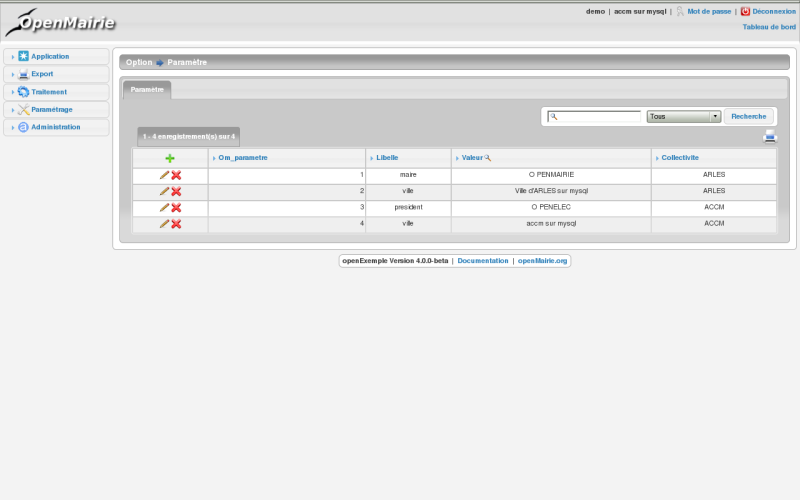
\includegraphics{tab_1.png}


\subsection{La requete SQL d'affichage}

Elle se trouve dans sql/type\_de\_sgbd/nom\_objet.inc

Les paramétres sont les suivants pour om\_parametre.inc

\begin{Verbatim}[commandchars=@\[\]]
@$serie=15;                                      Nombre d'enregistrement par page

@$ico="../img/ico@_application.png";              Icone affiché

@$ent = @_("option")." -@textgreater[] ".@_("om@_parametre");    Titre du tableau

@$idz                                            affichage en haut du formulaire

@$table=DB@_PREFIXE."om@_parametre";               Table de référence
                                                (il peut y avoir une ou plusieurs jointure)
@$champAffiche=array('om@_parametre',
                    'libelle',
                    'valeur',
                    'om@_collectivite');

@$champRecherche=array('libelle','valeur');      Champs pour la recherche

@$tri="";                                        Critere de tri par défaut

@$edition="om@_parametre";                        edition pdf

@$sousformulaire= array()                        sous formulaire(s) associé(s)



autre exemple de sous formulaire avec om@_collectivite.inc

    @$sousformulaire=array('om@_etat',
                    'om@_lettretype',
                    'om@_parametre',
                    'om@_sousetat',
                    'om@_utilisateur');
\end{Verbatim}


\subsection{Le script scr/tab.php}

L'affichage se fait à partir du menu (voir \emph{framework/parametrage}) sous la forme

\begin{Verbatim}[commandchars=@\[\]]
tab.php?obj=om@_parametre

où obj = nom@_d@_objet
\end{Verbatim}


\subsection{Le composant openMairie}

tab.php utilise les méthodes d'om\_table.class.php qui est une classe d'openMairie

\begin{Verbatim}[commandchars=@\[\]]
php/openmairie/om@_table.class.php
\end{Verbatim}

\resetcurrentobjects
\hypertarget{--doc-framework/formulaire}{}

\hypertarget{formulaire}{}\section{Les formulaires}

Les formulaires se construisent sur la base de la classe
formulairedyn.class.php d'openMairie

Cette classe fait appel a des sous programmes generiques pour certains
controles au travers de script js/formulairedyn.js


\subsection{Les methodes de formulairedyn.class.php}

La classe formulaire.class.php a les méthodes suivantes :

Les méthodes sur les controles du formulaire

\begin{Verbatim}[commandchars=@\[\]]
Hiddenstatic -@textgreater[] Champ non modifiable  Valeur récupéré par le formulaire
Hiddenstaticdate -@textgreater[] date non modifiable Valeur récupéré par le formulaire
statiq -@textgreater[] Valeur non modifiable
date -@textgreater[] date modifiable  js/calendrier
select -@textgreater[] Controle select
selectdisabled -@textgreater[] Controle select non modifiable
Text -@textgreater[] Controle text
hidden -@textgreater[] Controle non visible avec valeur conservée
password -@textgreater[] Controle password
Textdisabled -@textgreater[] Controle text non modifiable
comboG -@textgreater[] Appel à un programme de correspondance à une table
           Cas ou il y a une grosse table en correspondance
           spg/combo
ComboD -@textgreater[] Appel à un programme de correspondance à une table
           Cas ou il y a une grosse table en correspondance
           spg/combo
Upload -@textgreater[] spg/upload et spg/voir.php
textarea
textarea@_html
localisation -@textgreater[] spg/localisation.php
rvb -@textgreater[] spg/rvb.php
\end{Verbatim}

Les  méthodes de construction et d affichage

\begin{Verbatim}[commandchars=@\[\]]
afficher() affichage des champs (appelle par dbformdyn.class.php : methode formulaire
        -@textgreater[] afficherChampRegroupe() affichage des champs par regroupement / groupement
        -@textgreater[] afficherChamp() affichage de champ sans regroupe
recupererPostvarsousform() et recuperePostVar():
                recupèrent des variables apres validation
enpied() presentation
\end{Verbatim}

Les méthodes assesseurs changent les valeurs des proprietes de l'objet form (formulaire)

\begin{Verbatim}[commandchars=@\[\]]
setType()
setVal()
setLib()
setSelect()
setTaille()
setMax()
setOnchange()
setKeyup()
setOnclick()
setSelect()
setGroupe()
    D premier champ du groupe
    G champ groupe
    F dernier champ du groupe
setRegroupe()
    D premier champ du fieldset
    G champ dans le fieldset
    F dernier champ du fieldset
\end{Verbatim}

et enfin les méthodes de date

\begin{Verbatim}[commandchars=@\[\]]
dateAff(@$val)
\end{Verbatim}


\subsubsection{Les sous programmes génériques}

Les sous programmes génériques sont des sous programmes associés aux contrôles
du formulaire et appellés par eux par un script js dans js/formulairedyn.js

Les sous programmes génériques sont stockés dans le répertoire /spg.

\textbf{spg/combo.php}

Ce programme est appellé par le contrôle comboD, comboG, comboD2, comboG2
\begin{quote}

le paramétrage se fait dans les fichiers

\begin{Verbatim}[commandchars=@\[\]]
dyn@PYGbe[/]comboparametre@PYGbe[.]inc@PYGbe[.]php
dyn@PYGbe[/]comboretour@PYGbe[.]inc@PYGbe[.]php
dyn@PYGbe[/]comboaffichage@PYGbe[.]inc@PYGbe[.]php
\end{Verbatim}
\end{quote}

\textbf{spg/localisation.php} et js/localisation.js
\begin{quote}

ce programme est liée au contrôle formulaire ``localisation''
\end{quote}

\textbf{spg/voir.php}
\begin{quote}

Ce script est associé au contrôle ``upload''

Ce sous programme permet de visualiser un fichier téléchargé
sur le serveur (pdf ou image)
\end{quote}

\textbf{spg/upload.php}
\begin{quote}

Ce script utilise la classe php/openmairie/upload.class.php (composant openMairie)

Le paramétrage des extensions téléchargeables se fait dans le fichier autorise dans dyn/config.inc.php
\end{quote}

\textbf{spg/rvb.php} et js/rvb.js
\begin{quote}

Ce script est associé au contrôle ``rvb'' et permet l'accès à une palette de couleur
pour récupérer un code couleur rvb
\end{quote}


\subsubsection{le script scr/form.php}

form.php est le programme appellant d'un formulaire par rapport à un objet
métier(om\_parametre) et un identifiant (2)

form.php affiche le formulaires et éventuellement les sous formulaires (soustab.php et sousform.php)

exemple

\begin{Verbatim}[commandchars=@\[\]]
form.php?obj=om@_parametre@&idx=2
\end{Verbatim}


\subsubsection{Les nouvelles utilisations dans les objets metiers (openMairie 4)}

openMairie4 apporte de nouvelles fonctions qu'il est utile d'implémenter dans
les objets métiers

\textbf{récuperer le type de la base} depuis l'objet db : \$db-\textgreater{}phptype

\begin{Verbatim}[commandchars=@\[\]]
if(file@_exists ("../sql/".@$db-@textgreater[]phptype."/".@$this-@textgreater[]table.".form.inc"))/
                /include ("../sql/".@$db-@textgreater[]phptype."/".@$this-@textgreater[]table.".form.inc");/
\end{Verbatim}

\textbf{récuperer une erreur dans la base}

om4

\begin{Verbatim}[commandchars=@\[\]]
database::isError(@$res); // (@$res,true) = sans die
\end{Verbatim}

ce code remplace le code om3 (deprecated)

\begin{Verbatim}[commandchars=@\[\]]
//   if (DB :: isError(@$res))
//            @$this-@textgreater[]erreur@_db(@$res-@textgreater[]getDebugInfo(),@$res-@textgreater[]getMessage(),'');
//    else
//    {
//    if (@$DEBUG == 1)
//            echo "La requ@&ecirc;te de mise @&agrave; jour est effectu@&eacute;e.@textless[]br@textgreater[]";
\end{Verbatim}

\resetcurrentobjects
\hypertarget{--doc-framework/methode}{}

\hypertarget{methode}{}\section{La méthode}

Il est décrit ici la méthode pour la création d' objets métiers:

Le développement consiste à créer des objets métier (/obj) qui surchargent
la classe abstraite  dbformdyn.class.php et à modifier les valeurs par défaut
des variables dans les fichiers sql (nom\_objet.inc et nom\_objet.form.inc)

Voir aussi le \emph{générateur} pour automatiser les scripts métier.


\subsection{Surcharger les classes openMairie}

Il vaut mieux utiliser le générateur pour initialiser les classes metiers.

Le générateur surcharge la classe dbformdyn.class.php par rapport aux informations de la base

\begin{Verbatim}[commandchars=@\[\]]
classe abstraite @textless[]- classe metier generee @textless[]- classe metier 1 @textless[]- classe metier 2 ...
openMairie             depuis la base


dbformdyn.class.php @textless[]- gen/obj/nom@_objet.class.php @textless[]- obj/nom@_objet.class.php
\end{Verbatim}

Exemple avec concession d'openCimetiere

\begin{Verbatim}[commandchars=@\[\]]
dbformdyn.class.php  @textless[]- gen/obj/emplacement.class.php @textless[]-/obj/emplacement.class.php @textless[]- /obj/concession.class.php
\end{Verbatim}


\subsection{Modifier les valeurs par défaut}

Il est décrit ici les valeurs par défaut dans php/dbformdyn.class.php
qui est une classe d'openMairie.

Les valeurs suivantes sont mises par defaut afin de pouvoir construire rapidemment un formulaire

\begin{Verbatim}[commandchars=@\[\]]
valeur par defaut
   en ajout = initialisation vide

type par defaut
   type text pour ajout et modification
   type hiddenstatic pour suppression

libelle par défaut :
   Libellé = nom du champ dans le SGBD

taille et max d un champ
   Taille et max = longueur du champ dans le SGBD

les regroupements et groupements de champs sont vides

les fonctions javascript ne sont pas utilisées
\end{Verbatim}


\subsection{Modifier les valeurs par defaut par les méthodes assesseurs}

Elles se font dans la classe obj/nom\_objet.class.php

Les valeurs par défaut sont modifiées par la méthode setVal(nomduchamp, nouvelle valeur)

Les types par défaut sont modifiés par la méthode setType(nomduchamp, nouveau type)

Les longueurs d affichage par défaut sont modifiées par la méthode setTaille(nomduchamp, nouvelle valeur)

Les maximums autorisés par défaut sont modifiés par la méthode setMax(nomduchamp, nouvelle valeur)

Les libelles de champ par défaut sont modifiés par la méthode setLib(nomduchamp, nouvelle valeur)

Les scripts javascript sont appellés dans la méthode setOnchange()

Voir framework/formulaire


\subsection{La class dbformdyn.class.php}

dbform.class.php  est une classe openMairie

La classe abstraite dbform gère l’interface entre l'objet métier et la base de données connectée via DBPEAR.

Les méthodes principales sont les suivantes :
\begin{itemize}
\item {} 
orientées sgbd

\begin{Verbatim}[commandchars=@\[\]]
constructeur
ajouter : Ajoute un objet
Modifier : Modifie un objet
Supprimer : Supprime un objet
Verifier : Contrôle un objet
Clesecondaire : Contrôle les cles secondaires
triggers avant/apres ajout/modification/suppression
\end{Verbatim}

\item {} 
orientees Formulaire

\begin{Verbatim}[commandchars=@\[\]]
Formulaire : Constitue le formulaire et fait appel à formulaire.dyn.class.php
sousFormulaire : Constitue le sousformulaire -@textgreater[] appel à formulaire.dyn.class.php
Message : Retourne le message d erreur (contrôle php)
bouton : Affiche le bouton
Retour : gére le retour à une interface php en fin de saisie
sousformulaireRetour : gére le retour à une interface php en fin de saisie de sous formulaire
setType : Envoi au formulaire les type de champ
setVal : Envoi au formulaire les valeurs par défaut
setValSousformulaire : Envoi au sousformulaire les valeurs par défaut
setlib : Envoi au formulaire les libellés de champs
setTaille : Envoi au formulaire la taille du champ
setMax : Envoi au formulaire la taille maximum autorisée du champ
setSelect : Envoi au formulaire les champs select à afficher
setOnchange : Envoi au formulaire les controles javascript à effectuer en cas de changement de données dans le champ
setGroupe : Envoi au formulaire le regroupement de champ par ligne
setRegroupe : Envoi au formulaire un fieldset
\end{Verbatim}

\item {} 
des fonctions de traitement de champ heure et date:

\begin{Verbatim}[commandchars=@\[\]]
DateDB : transforme les dates affichées en date pour base de données
HeureDB : controle du champs heure saisi 00 ou 00:00 ou 00:00:00
DateSystemeDB : mise au format base de donnees de la date systeme
DatePHP : controle et transforme la date saisie (jj/mm/aaaa) en date format PHP
\end{Verbatim}

\item {} 
des fonctions pour faire des calculs

\begin{Verbatim}[commandchars=@\[\]]
AnneePHP : controle et recupere l’année de la date saisie (jj/mm/aaaa)
MoisPHP : controle et recupere le mois de la date saisie (jj/mm/aaaa)
JourPHP : controle et recupere le jour de la date saisie (jj/mm/aaaa)
\end{Verbatim}

\end{itemize}

La classe dbformdyn.class.php fait appel à la classe formulaire.dyn.class.php pour afficher le formulaire.

Il est créé 2 objets :
\begin{itemize}
\item {} 
un objet db qui fait la connexion avec la base

\item {} 
un objet form qui décrit le formulaire

\end{itemize}


\subsection{L'objet db}

db est l'objet de connexion a la base dont les proprietes sont les suivantes

\begin{Verbatim}[commandchars=@\[\]]
DB@_pgsql Object

(
@PYGZlb[]phptype@PYGZrb[] =@textgreater[] pgsql
    @PYGZlb[]dbsyntax@PYGZrb[] =@textgreater[] pgsql
    @PYGZlb[]features@PYGZrb[] =@textgreater[] Array (
                    @PYGZlb[]limit@PYGZrb[] =@textgreater[] alter
                    @PYGZlb[]new@_link@PYGZrb[] =@textgreater[] 4.3.0
                    @PYGZlb[]numrows@PYGZrb[] =@textgreater[] 1
                    @PYGZlb[]pconnect@PYGZrb[] =@textgreater[] 1
                    @PYGZlb[]prepare@PYGZrb[] =@textgreater[]
                    @PYGZlb[]ssl@PYGZrb[] =@textgreater[] 1
                    @PYGZlb[]transactions@PYGZrb[] =@textgreater[] 1 )
                    @PYGZlb[]errorcode@_map@PYGZrb[] =@textgreater[] Array ( )
                    @PYGZlb[]connection@PYGZrb[] =@textgreater[] Resource id @#19
                    @PYGZlb[]dsn@PYGZrb[] =@textgreater[] Array (
                            @PYGZlb[]phptype@PYGZrb[] =@textgreater[] pgsql
                            @PYGZlb[]dbsyntax@PYGZrb[] =@textgreater[] pgsql
                            @PYGZlb[]username@PYGZrb[] =@textgreater[] postgres
                            @PYGZlb[]password@PYGZrb[] =@textgreater[] postgres
                            @PYGZlb[]protocol@PYGZrb[] =@textgreater[] tcp
                            @PYGZlb[]hostspec@PYGZrb[] =@textgreater[] localhost
                            @PYGZlb[]port@PYGZrb[] =@textgreater[] 5432
                            @PYGZlb[]socket@PYGZrb[] =@textgreater[]
                            @PYGZlb[]database@PYGZrb[] =@textgreater[] sig
                            @PYGZlb[]title@PYGZrb[] =@textgreater[] Openmairie Exemple PostGreSQL schema SIG
                            @PYGZlb[]formatdate@PYGZrb[] =@textgreater[] AAAA-MM-JJ
                            @PYGZlb[]schema@PYGZrb[] =@textgreater[] openmairie
                    )
                    @PYGZlb[]autocommit@PYGZrb[] =@textgreater[] 1
                    @PYGZlb[]transaction@_opcount@PYGZrb[] =@textgreater[] 0
                    @PYGZlb[]affected@PYGZrb[] =@textgreater[] 0
                    @PYGZlb[]row@PYGZrb[] =@textgreater[] Array (@PYGZlb[]20@PYGZrb[] =@textgreater[] 10 )
                    @PYGZlb[]@_num@_rows@PYGZrb[] =@textgreater[] Array ( @PYGZlb[]20@PYGZrb[] =@textgreater[] 10 )
                    @PYGZlb[]fetchmode@PYGZrb[] =@textgreater[] 1
                    @PYGZlb[]fetchmode@_object@_class@PYGZrb[] =@textgreater[] stdClass
                    @PYGZlb[]was@_connected@PYGZrb[] =@textgreater[]
                    @PYGZlb[]last@_query@PYGZrb[] =@textgreater[] select * from openmairie.om@_parametre where om@_collectivite=2
                    @PYGZlb[]options@PYGZrb[] =@textgreater[] Array (
            @PYGZlb[]result@_buffering@PYGZrb[] =@textgreater[] 500
                            @PYGZlb[]persistent@PYGZrb[] =@textgreater[]
                            @PYGZlb[]ssl@PYGZrb[] =@textgreater[]
            @PYGZlb[]debug@PYGZrb[] =@textgreater[] 2
            @PYGZlb[]seqname@_format@PYGZrb[] =@textgreater[] @%s@_seq
            @PYGZlb[]autofree@PYGZrb[] =@textgreater[]
            @PYGZlb[]portability@PYGZrb[] =@textgreater[] 63
            @PYGZlb[]optimize@PYGZrb[] =@textgreater[] performance
            )
                    @PYGZlb[]last@_parameters@PYGZrb[] =@textgreater[] Array ( )
                    @PYGZlb[]prepare@_tokens@PYGZrb[] =@textgreater[] Array ( )
                    @PYGZlb[]prepare@_types@PYGZrb[] =@textgreater[] Array ( )
                    @PYGZlb[]prepared@_queries@PYGZrb[] =@textgreater[] Array ( )
                    @PYGZlb[]@_last@_query@_manip@PYGZrb[] =@textgreater[]
                    @PYGZlb[]@_next@_query@_manip@PYGZrb[] =@textgreater[]
                    @PYGZlb[]@_debug@PYGZrb[] =@textgreater[]
                    @PYGZlb[]@_default@_error@_mode@PYGZrb[] =@textgreater[]
                    @PYGZlb[]@_default@_error@_options@PYGZrb[] =@textgreater[]
                    @PYGZlb[]@_default@_error@_handler@PYGZrb[] =@textgreater[]
                    @PYGZlb[]@_error@_class@PYGZrb[] =@textgreater[] DB@_Error
                    @PYGZlb[]@_expected@_errors@PYGZrb[] =@textgreater[] Array ( )
)
\end{Verbatim}


\subsection{L'objet form}

form est l'objet formulaire dont les proprietes sont les suivantes

\begin{Verbatim}[commandchars=@\[\]]
formulaire Object (
    @PYGZlb[]enteteTab@PYGZrb[] =@textgreater[]
    @PYGZlb[]val@PYGZrb[] =@textgreater[] Array (
            @PYGZlb[]om@_parametre@PYGZrb[] =@textgreater[] 1
            @PYGZlb[]libelle@PYGZrb[] =@textgreater[] maire
            @PYGZlb[]valeur@PYGZrb[] =@textgreater[] O PENMAIRIE
            @PYGZlb[]om@_collectivite@PYGZrb[] =@textgreater[] 1 )
    @PYGZlb[]type@PYGZrb[] =@textgreater[] Array (
            @PYGZlb[]om@_parametre@PYGZrb[] =@textgreater[] text
            @PYGZlb[]libelle@PYGZrb[] =@textgreater[] text
            @PYGZlb[]valeur@PYGZrb[] =@textgreater[] text
            @PYGZlb[]om@_collectivite@PYGZrb[] =@textgreater[] text )
    @PYGZlb[]taille@PYGZrb[] =@textgreater[] Array (
            @PYGZlb[]om@_parametre@PYGZrb[] =@textgreater[] 11
            @PYGZlb[]libelle@PYGZrb[] =@textgreater[] 20
            @PYGZlb[]valeur@PYGZrb[] =@textgreater[] 50
            @PYGZlb[]om@_collectivite@PYGZrb[] =@textgreater[] 11 )
    @PYGZlb[]max@PYGZrb[] =@textgreater[] Array (
            @PYGZlb[]om@_parametre@PYGZrb[] =@textgreater[] 11
            @PYGZlb[]libelle@PYGZrb[] =@textgreater[] 20
            @PYGZlb[]valeur@PYGZrb[] =@textgreater[] 50
            @PYGZlb[]om@_collectivite@PYGZrb[] =@textgreater[] 11 )
    @PYGZlb[]lib@PYGZrb[] =@textgreater[] Array (
            @PYGZlb[]om@_parametre@PYGZrb[] =@textgreater[] Om@_parametre
            @PYGZlb[]libelle@PYGZrb[] =@textgreater[] Libelle
            @PYGZlb[]valeur@PYGZrb[] =@textgreater[] Valeur
            @PYGZlb[]om@_collectivite@PYGZrb[] =@textgreater[] Om@_collectivite )
    @PYGZlb[]groupe@PYGZrb[] =@textgreater[] Array (
            @PYGZlb[]om@_parametre@PYGZrb[] =@textgreater[]
            @PYGZlb[]libelle@PYGZrb[] =@textgreater[]
            @PYGZlb[]valeur@PYGZrb[] =@textgreater[]
            @PYGZlb[]om@_collectivite@PYGZrb[] =@textgreater[] )
    @PYGZlb[]select@PYGZrb[] =@textgreater[] Array (
            @PYGZlb[]om@_parametre@PYGZrb[] =@textgreater[]  Array (@PYGZlb[]0@PYGZrb[] =@textgreater[] @PYGZlb[]1@PYGZrb[] =@textgreater[] )
            @PYGZlb[]libelle@PYGZrb[] =@textgreater[] Array ( @PYGZlb[]0@PYGZrb[] =@textgreater[] @PYGZlb[]1@PYGZrb[] =@textgreater[] )
            @PYGZlb[]valeur@PYGZrb[] =@textgreater[] Array ( @PYGZlb[]0@PYGZrb[] =@textgreater[] @PYGZlb[]1@PYGZrb[] =@textgreater[] )
            @PYGZlb[]om@_collectivite@PYGZrb[] =@textgreater[] Array ( @PYGZlb[]0@PYGZrb[] =@textgreater[] @PYGZlb[]1@PYGZrb[] =@textgreater[] ) )
    @PYGZlb[]onchange@PYGZrb[] =@textgreater[] Array (
            @PYGZlb[]om@_parametre@PYGZrb[] =@textgreater[]
            @PYGZlb[]libelle@PYGZrb[] =@textgreater[]
            @PYGZlb[]valeur@PYGZrb[] =@textgreater[]
            @PYGZlb[]om@_collectivite@PYGZrb[] =@textgreater[] )
    @PYGZlb[]onkeyup@PYGZrb[] =@textgreater[] Array (
            @PYGZlb[]om@_parametre@PYGZrb[] =@textgreater[]
            @PYGZlb[]libelle@PYGZrb[] =@textgreater[]
            @PYGZlb[]valeur@PYGZrb[] =@textgreater[]
            @PYGZlb[]om@_collectivite@PYGZrb[] =@textgreater[] )
    @PYGZlb[]onclick@PYGZrb[] =@textgreater[] Array (
            @PYGZlb[]om@_parametre@PYGZrb[] =@textgreater[]
            @PYGZlb[]libelle@PYGZrb[] =@textgreater[]
            @PYGZlb[]valeur@PYGZrb[] =@textgreater[]
            @PYGZlb[]om@_collectivite@PYGZrb[] =@textgreater[] )
    @PYGZlb[]regroupe@PYGZrb[] =@textgreater[]
    @PYGZlb[]correct@PYGZrb[] =@textgreater[]
)
\end{Verbatim}

\resetcurrentobjects
\hypertarget{--doc-framework/edition}{}

\hypertarget{edition}{}\section{Les éditions}

Les éditions sont accessibles dans le menu par :
\begin{itemize}
\item {} 
administration -\textgreater{} etat

\item {} 
administration -\textgreater{} sousetat

\item {} 
administration -\textgreater{} lettretype

\end{itemize}

Depuis la version 4 d'openMairie, les editions sont conservées dans 3 tables :
\begin{itemize}
\item {} 
om\_etat : pour les états

\item {} 
om\_sousetat : pour les sous etats

\item {} 
om\_lettretype : pour les lettres types

\end{itemize}

Cette modification a été faite pour pouvoir gérer la multi collectivité.

Par contre, les tableaux pdf sont stockés dans un fichier : nom\_objet.pdf.inc


\subsection{Actif, non actif}

Les sous etats sont liés a un ou plusieurs état

Les états, sous etats, et lettre type peuvent être actif ou non actif

Par défaut sont pris en compte :

1 - l'édition  ``actif'' de la collectivite

2 - l'édition ``actif'' de la multicollectivite

3 - l'édition ``non actif'' de la multicollectivite

Les editions non actifs d'une collectivite ne sont pas pris en compte


\subsection{Paramétrer des etats}

Il est conseillé d utiliser l'assistant état du generateur

Les paramètres sont les suivants

\begin{Verbatim}[commandchars=@\[\]]
orientation portrait ou paysage
format="A4", A3
position et nom  du logo
titre de l etat
position et caractéristiques du titre
corps de l etat
position et caractéristiques du corps
la requete SQL
les sous etats associés et les caractéristiques
\end{Verbatim}

Pour le corps, le titre et la requete sql, les zones entre crochets (exemple {[}nom{]}) sont les champs selectionnés par la requete.

Les variables commençant par ``\&'' sont définies dans dyn/varpdf.inc (exemple \&aujourdhui)
et dans la table om\_parametre.


\subsection{Paramétrer des sous etats}

Il est conseillé d utiliser l'assistant sousetat du générateur

Les paramétres  sont les suivants

\begin{Verbatim}[commandchars=@\[\]]
texte et caractéristique du Titre
Intervalle avant et apres le tableau
Entete de tableau (nom de colone)
caracteristique du tableau
caracteristique des cellules
tatal, moyenne, nombre
requete sql
\end{Verbatim}

Pour le titre et la requete sql, les zones entre crochets sont les champs selectionnés par la requete.

Les variables commençant par ``\&'' sont définies dans dyn/varpdf.inc (exemple \&aujourdhui)
et dans la table om\_parametre


\subsection{Paramétrer des lettres type}

Il est conseillé d utiliser l assistant lettretype du generateur

Les paramétres sont les suivants

\begin{Verbatim}[commandchars=@\[\]]
orientation portrait ou paysage
format="A4", A3
position et nom  du logo
titre de la lettre
position et caractéristiques du titre
corps de la lettre
position et caractéristiques du corps
la requete SQL
\end{Verbatim}

Pour le corps, le titre et la requete sql, les zones entre crochets  sont les champs selectionnés par la requete.

Les variables commençant par ``\&'' sont définies dans dyn/varlettretypepdf.inc (exemple \&aujourdhui)
et dans la table om\_parametre


\subsection{Parametrer des edition pdf}

Un etat pdf peut être généré par le generateur (option)

L'edition est paramétrée dans un fichier sql/sgbd/nom\_objet.pdf.inc et dans la

Les paramétres sont les suivants

\begin{Verbatim}[commandchars=@\[\]]
texte et caractéristique du Titre
Entete de tableau (nom de colone)
caracteristique du tableau
caracteristique des cellules
tatal, moyenne, nombre
requete sql
\end{Verbatim}

Pour le titre et la requete sql, les zones entre crochets sont les champs selectionnés par la requete.

Les variables commençant par ``\&'' sont définies dans dyn/varpdf.inc (exemple \&aujourdhui)
et dans la table om\_parametre


\subsection{Parametrer les etiquettes}

Les zones entre crochets  sont les champs selectionnés par la requete.
La variable  \&aujourdhui sont définies dans dyn/varetiquettepdf.inc et dans la
table om\_parametre

Il y aura une integration depuis l utilisation d'openPersonnalite dans la version openMairie 4.0.1..


\subsection{L'éditeur WYSIWYG}

Un editeur est prevu dans la prochaine version openMairie 4.0.1


\subsection{Les scripts PDF}

Les scripts sont dans le répertoire  \textbf{pdf/} et sont  appellés par le framework sous la forme

\begin{Verbatim}[commandchars=@\[\]]
pdfetat.php?obj=nom@_etat@&idx=enregistrement@_a@_editer
\end{Verbatim}

les scripts sont les suivants

\begin{Verbatim}[commandchars=@\[\]]
pdfetat.php : etat et sous etat
pdf.php : edition pdf
pdfetiquette.php : etiquette
pdflettretype.php
\end{Verbatim}

pdfEtiquette sera repris dans la version 4.0.1 d'openMairie

\textbf{specifique openCourrier pour ecriture sur pdf}

\begin{Verbatim}[commandchars=@\[\]]
fpdf@_tpl@PYGbe[.]php
fpdi@PYGbe[.]php
fpdi2tcpdf@_bridge@PYGbe[.]php
fpdi@_pdf@_parser@PYGbe[.]php
histo@PYGbe[.]htm
pdf@_context@PYGbe[.]php
pdf@_parser@PYGbe[.]php
testfpdi@PYGbe[.]php
\end{Verbatim}

Il n est pas prévu d integration dans la prochaine version


\subsection{composants}

Les composants php sont stockés en \textbf{php/}

\emph{/openmairie}

Les scripts ci dessous sont les classes qui interfacent openmairie avec fpdf

\begin{Verbatim}[commandchars=@\[\]]
fpdf@_etat@PYGbe[.]php
fpdf@_etiquette@PYGbe[.]php
db@_fpdf@PYGbe[.]php
\end{Verbatim}

\emph{/fpdf}
\begin{quote}

A ce niveau se situe le composant fpdf
\end{quote}

\emph{/phpmailer}
\begin{quote}

la gestion de mail est EN TEST avec openPersonnalite et sera intégré dans  openMairie 4.0.1
\end{quote}

Les composants javascript sont stockés dans le repertoire \textbf{lib/}

\emph{/tinymce}
\begin{quote}

est l'editeur wisiwig   EN TEST sur openRecensement et qui sera intégré dans openmairie 4.0.1)
\end{quote}

\resetcurrentobjects
\hypertarget{--doc-framework/reqmo}{}

\hypertarget{reqmo}{}\section{Les requêtes memorisées}

les requêtes mémorisées permettent au développeur de fournir un ensemble de requêtes :
\begin{itemize}
\item {} 
mémorisées

\item {} 
accessible dans le menu export -\textgreater{} requêtes

\item {} 
paramétrables par l'utilisateur

\item {} 
permettant un affichage html en tableau ou un transfert au format csv sur tableur (choix du séparateur à l utilisateur)

\end{itemize}

menu export-\textgreater{} requete

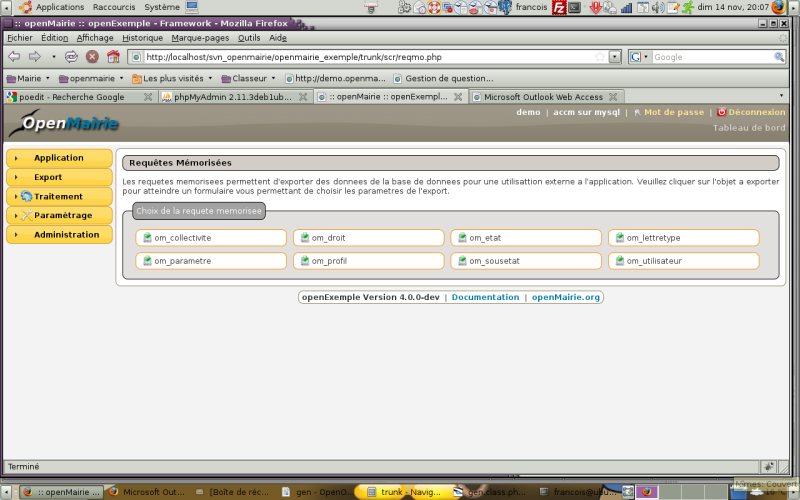
\includegraphics{reqmo_1.png}


\subsection{Description du parametrage}

\textbf{Les parametres de reqmo  sont :}
\begin{quote}

\$reqmo{[}'libelle'{]} contient le libéllé affiché en haut

\$reqmo{[}'sql'{]} contient la requete SQL.

Dans la requete, les paramétres sont mis entre {[}{]}

et ils sont définis en dessous  sous la forme reqmo{[}parametre{]}=.
\begin{quote}

``checked'' : la colonne est affiché ou non

``un tableau'' array(a,b) et le choix a ou b est donné à l utilisateur de requete

``une requete sql'' : le choix se fait dans la table du select
\end{quote}
\end{quote}

La requete executée est celle qui est reconstituée avec les zones sasisies par l'utilisateur

Enfin, l utilisateur choisi soit un affichage soit en tableau, soit en csv avec un choix de séparateur.

Il n y a pas d'outil de fabrication de requête à part l'option du générateur
(voir chapître sur le \emph{générateur})


\subsection{Exemple}

\textbf{voies sous openCimetiere}

\begin{Verbatim}[commandchars=@\[\]]
@$reqmo@PYGZlb[]'libelle'@PYGZrb[]=" Voies par cimetiere ";

@$reqmo@PYGZlb[]'sql'@PYGZrb[]=" select voie,voietype,voielib,
                @PYGZlb[]zonetype@PYGZrb[],@PYGZlb[]zonelib@PYGZrb[],
                @PYGZlb[]cimetierelib@PYGZrb[]
                from voie
                inner join zone
                on voie.zone=zone.zone
                inner join cimetiere
                on zone.cimetiere=cimetiere.cimetiere
                where cimetiere.cimetiere = @PYGZlb[]cimetiere@PYGZrb[] order by @PYGZlb[]tri@PYGZrb[]";

@$reqmo@PYGZlb[]'tri'@PYGZrb[]= array('voielib',
                 'zonelib'
                 );
@$reqmo@PYGZlb[]'zonetype'@PYGZrb[]="checked";
@$reqmo@PYGZlb[]'zonelib'@PYGZrb[]="checked";
@$reqmo@PYGZlb[]'cimetierelib'@PYGZrb[]="checked";
@$reqmo@PYGZlb[]'cimetiere'@PYGZrb[]="select cimetiere,concat(cimetiere,' ',
        cimetierelib) from cimetiere";
\end{Verbatim}

\resetcurrentobjects
\hypertarget{--doc-framework/acces}{}\begin{quote}
\hypertarget{acces}{}\end{quote}


\section{La gestion des accès}

Le framework fournit un gestionnaire d'accés accessible dans le menu à :
\begin{itemize}
\item {} 
administration -\textgreater{} profil

\item {} 
administration -\textgreater{} droit

\item {} 
administration -\textgreater{}utilisateur

\end{itemize}

Les accès sont conservés dans des tables.


\subsection{Les tables}

La gestion des accès est gérée avec 3 tables :

\textbf{om\_profil} : gestion des profils

\begin{Verbatim}[commandchars=@\[\]]
administrateur
super utilisateur
utilisateur
utilisateur limite
consultation
\end{Verbatim}

\textbf{om\_droit}: la gestion des droits affecte un profil suivant chaque :
\begin{quote}

objet métier : \$obj om\_collectivite, om\_parametre ...

chaque rubrique du menu :

voir paramétrage menu : tableau Rubrik  right = ``om\_parametre''
\end{quote}

\textbf{om\_utilisateur} : cette table permet de donner un login, un mot de passe
et un profil à chaque utilisateur

Diagramme de classe

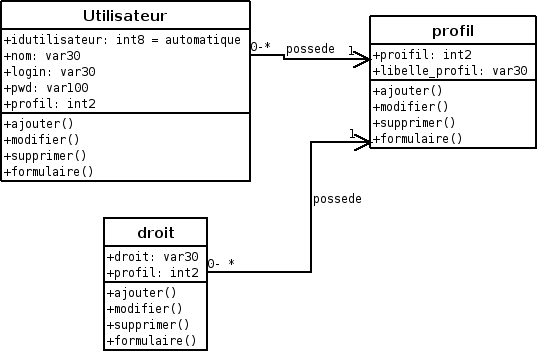
\includegraphics{acces_1.png}


\subsection{Les règles}
\begin{itemize}
\item {} 
le droit sur un objet porte le nom de l'objet

\item {} 
chaque profil a acces a tous les droits des profils d un niveau inférieur

\item {} 
l'adminitrateur a acces à tout.

\end{itemize}


\subsection{Les login et logout}

Le login se fait par le script \emph{scr/login.php}

login.php valorise les variables sessions  permettant la gestion des acces et securites:

\begin{Verbatim}[commandchars=@\[\]]
@$@_SESSION@PYGZlb[]'profil'@PYGZrb[] = @$profil;
@$@_SESSION@PYGZlb[]'nom'@PYGZrb[] = @$nom;
@$@_SESSION@PYGZlb[]'login'@PYGZrb[] = @$login;
\end{Verbatim}

La deconnexion se fait avec le script  \emph{scr/logout}

Le changement de mot de passe se fait avec le script  \emph{scr/password.php}

L'accès au changement de passe se fait par défaut dans le menu haut
(voir framework/paramétrage)


\subsection{Les utilitaires}

La gestion des droits d'acces se fait dans les méthodes des utilitaires
\begin{quote}

php/openmairie/om\_appication.class.php (composant openMairie)

obj/utils.class.php
\end{quote}

(\emph{voir framework/utilitaire})

\resetcurrentobjects
\hypertarget{--doc-framework/ergonomie}{}

\hypertarget{ergonomie}{}\section{L'ergonomie}

Depuis la version openMairie 4, il est décidé d'utiliser l'ergonomie de jquery.


\subsection{Le composant jquery}

Les skins jquery peuvent être rajoutés dans le repertoire /lib/jquery\_ui.

Le changement de skin se fait dans le fichier dyn/config.inc.php

\emph{voir framework/parametrage}


\subsection{Les feuilles de style}

Les feuilles de style sont stockées dans le repertoire css/ et sont cascadables

\begin{Verbatim}[commandchars=@\[\]]
main.css : principale openMairie
    specific.css : specifique a l application
        specific@_om@_... : suivant la feuille de style jquery choisi dans l application (1)
\end{Verbatim}


\subsection{La mise en oeuvre dans les scripts}

\emph{voir framework/utilitaire}

\resetcurrentobjects
\hypertarget{--doc-framework/utilitaire}{}

\hypertarget{utilitaire}{}\section{Les utilitaires}

Les méthodes spécifiques à l'application sont dans obj/utils.class.php
qui héritent de la class om\_application.class.php d `openmairie

Vous pouvez surcharger les classes d'om\_application.class.php dans utils.class.php

Exemple : surcharge de la méthode login() pour conserver le service d'un utilisateur
en variable session dans openCourrier.

Ces classes contiennent les méthodes utilisées par le framework mais
qui peuvent vous aider à développer les scripts complémentaires de votre application.

Les scripts complémentaires peuvent être créer pour :
\begin{itemize}
\item {} 
faire un traitement en répertoire trt/ (remise à 0 d'un registre, archivage, export ....)

\item {} 
faire un sous programme spécifique en spg/ appellé par un formulaire (bible.php dans openCourrier)

\item {} 
faire une recherche avec un affichage particulier en scr/.

\end{itemize}


\subsection{Le tutorial}

Il est proposé ici de vous montrer comment réaliser ce script complémentaire

Le script commence obligatoirement par un appel à la bibliothèque utils.class.php et la creation d un objet \$f:

\begin{Verbatim}[commandchars=@\[\]]
require@_once "../obj/utils.class.php";
@$f = new utils(NULL,
            "courrier",
            @_("recherche"),
            "ico@_recherche.png",
            "recherche");
\end{Verbatim}

Les parametres de l'objet sont les suivants :
\begin{quote}

flag : si flag= Null affichage complete
\begin{quote}

nonhtml : pas d affichage

htmlonly : tout les elements externes html avec body vide
\end{quote}

right : droit géré en om\_droit - vide ne verifie pas

title : titre affiché

icon  : icone affiché

help  : aide affiché
\end{quote}

utils.class.php fait la Verification si l utilisateur est authentifié et si l utilisateur a le droit

Si le paramétre ``right'' est vide vous pouvez faire appel aux méthodes suivantes

\begin{Verbatim}[commandchars=@\[\]]
isAccredited() // a le droit ou pas
isAuthentified // si non authentifié, il est rejeté

@$f-@textgreater[]setRight(@$obj); // affecte un droit d acces
@$f-@textgreater[]isAuthorized(); //verification que l utilisateur accéde

// Affectation des variables en dehors du constructeur
@$f-@textgreater[]setTitle(@$ent);
@$f-@textgreater[]setIcon(@$ico);
@$f-@textgreater[]setHelp(@$obj);
@$f-@textgreater[]setFlag(NULL);

// affichage
@$f-@textgreater[]display();
\end{Verbatim}

Pour \textbf{executer une requête dans un fichier sql} vous devez stocker
votre requête dans le répertoire sql/type\_de\_sgbd/nom\_de\_requete.inc
afin de préserver la portabilité de vos travaux sur d'autres sgbd:

\begin{Verbatim}[commandchars=@\[\]]
// appel au fichier requête
include ("../sql/".@$f-@textgreater[]phptype."/courrier@_scr.inc");

// lancement de la requete sql@_courrier et test erreur
@$res=@$f-@textgreater[]db-@textgreater[]query(@$sql@_courrier);
@$f-@textgreater[]isDatabaseError(@$res);
\end{Verbatim}

Pour \textbf{parcourir les enregistrements} vous utilisez les méthodes dbpear suivantes:

\begin{Verbatim}[commandchars=@\[\]]
// du debut à la fin de la requête
while (@$row=@& @$res-@textgreater[]fetchRow(DB@_FETCHMODE@_ASSOC)){
    // j'affiche le champ courrier
     echo @$row@PYGZlb[]'courrier'@PYGZrb[];

}
\end{Verbatim}

Pour \textbf{ecrire dans la base} vous pouvez utiliser les méthodes insert ou update
mais vous pouvez utilisez la méthode autoexecute spécifique à db pear:

\emph{requête sql}

\begin{Verbatim}[commandchars=@\[\]]
@$sql = "INSERT INTO ... ";

@$res2 = @$f -@textgreater[] db -@textgreater[] query(@$sql);

@$f-@textgreater[]isDatabaseError(@$res2);
\end{Verbatim}

\emph{ou avec un tableau \$valF}

\begin{Verbatim}[commandchars=@\[\]]
@$obj = table

@$valF@PYGZlb[]@$obj@PYGZrb[]=@$f-@textgreater[] db -@textgreater[] nextId(DB@_PREFIXE.@$obj);

@$res1= @$f-@textgreater[] db -@textgreater[] autoExecute(DB@_PREFIXE.@$obj,@$valF,DB@_AUTOQUERY@_INSERT);

@$f-@textgreater[]isDatabaseError(@$res1);
\end{Verbatim}

Vous pouvez faire une \textbf{Description du role de la page} de la manière suivante

\begin{Verbatim}[commandchars=@\[\]]
@$description = @_("Cette page vous permet de .. ");

@$f-@textgreater[]displayDescription(@$description);
\end{Verbatim}

Un \textbf{message d erreur} s'affiche suivant :
\begin{quote}

\$class : qui est la classe css qui s'affiche sur l'element et qui peut être
\begin{quote}

``error'' : pour le message erreur

``valid'' : pour le message de validation
\end{quote}
\end{quote}

le \emph{code} est le suivant

\begin{Verbatim}[commandchars=@\[\]]
@$message = @_("Mot de passe actuel incorrect");
@$f-@textgreater[]displayMessage(@$class, @$message);
\end{Verbatim}

Pour afficher  un \textbf{fieldset}, le code est le suivant

\begin{Verbatim}[commandchars=@\[\]]
echo "@textless[]fieldset class=\"cadre ui-corner-all ui-widget-content\"@textgreater[]\n";

echo "\t@textless[]legend class=\"ui-corner-all ui-widget-content ui-state-active\"@textgreater[]";

echo @_("Courrier")."@textless[]/legend@textgreater[]";
    ...
echo "@textless[]/fieldset@textgreater[]
\end{Verbatim}

il peut être par défqut \emph{ouvert}

\begin{Verbatim}[commandchars=@\[\]]
echo "@textless[]fieldset class= ... collapsible\"@textgreater[]\n";
\end{Verbatim}

ou il peut être \emph{fermé}

\begin{Verbatim}[commandchars=@\[\]]
echo "@textless[]fieldset ... startClosed\"@textgreater[]\n";
\end{Verbatim}

Vous pouvez faire \textbf{appel a des scripts js complementaires} en utilisant la méthode

\begin{Verbatim}[commandchars=@\[\]]
@$f-@textgreater[]addHTMLHeadJs(array("../js/formulairedyn.js", "../js/onglet.js"));
\end{Verbatim}

Pour la \textbf{gestion des accents}, il est conseillé de ne pas mettre d accent dans
le code (utf8 au lieu de latin1-iso8859-1) et de mettre les accents dans la traduction

Pour définir le chemin par défaut pour l' ** upload de fichier**, il faut utiliser la méthode

\begin{Verbatim}[commandchars=@\[\]]
@$path=@$f-@textgreater[]getPathFolderTrs()
\end{Verbatim}


\subsection{Exemple}

Il est proposé de prendre l'exemple du traitement de la remise du registre
a 0 dans openCourrier

\begin{Verbatim}[commandchars=@\[\]]
// ENTETE NORMALISEE

/**
 * Cette page permet de remettre a 0 le registre
 *
 * @PYGZat[]package openmairie@_exemple
 * @PYGZat[]version SVN : @$Id: xxxx.php 311 2010-12-06 11:43:36Z xxxxx @$
 */


// CREATION DE L' OBJET @$f

require@_once "../obj/utils.class.php";
@$f = new utils(NULL, "traitement", @_("remise a 0 du registre"), "ico@_registre.png", "recherche");



// get
if (isset (@$@_GET@PYGZlb[]'validation'@PYGZrb[])){
   @$validation=@$@_GET@PYGZlb[]'validation'@PYGZrb[];
}else{
   @$validation=0;
}


/**
 * Description de la page
 */

@$description = @_("Cette page vous permet de remettre a 0 le numero de registre ".
                 "Ce traitement est a faire en debut d annee.");
@$f-@textgreater[]displayDescription(@$description);


// TEST VALIDATION
// SI = 0 affichage du numero de registre
// SI = 1 mise à 0 du registre et affichage du résultat

if(@$validation==0){
    @$validation=1;

    // REQUETE DU REGISTRE

    @$sql= "select id from registre@_seq" ;
    @$res1=@$f-@textgreater[]db-@textgreater[]getOne(@$sql);
    @$f-@textgreater[]isDatabaseError(@$res1);

    // AFFICHAGE DANS UN FIELDSET

    echo "@textless[]fieldset class=\"cadre ui-corner-all ui-widget-content\"@textgreater[]\n";
    echo "\t@textless[]legend class=\"ui-corner-all ui-widget-content ui-state-active\"@textgreater[]";
    echo @_("Registre ")."@textless[]/legend@textgreater[]";
    if (@$res1!=0){
        echo "@textless[]br@textgreater[]".@_("le dernier no du registre est")." : @&nbsp;@&nbsp;".@$res1."@&nbsp;@&nbsp;";
    }else{
        echo "@textless[]br@textgreater[]".@_("vous avez deja fait une remise a 0")."@textless[]br@textgreater[]";
    }
    echo "@textless[]form method=\"POST\" action=\"num@_registre.php?validation=".
    @$validation."\" name=f1@textgreater[]";
    echo "@textless[]/fieldset@textgreater[]";

    // BOUTON DE VALIDATION
    echo "\t@textless[]div class=\"formControls\"@textgreater[]";
    echo "@textless[]input type='submit' value='".@_("remise a 0 du registre").
          "@&nbsp;' @textgreater[]";
    echo "@textless[]/div@textgreater[]";
    echo "@textless[]/form@textgreater[]";

}else { // validation=1

    // VALORISATION DE @$valF
    @$valF=array();
    @$valF@PYGZlb[]'id'@PYGZrb[]=0;

    // REQUETE MISE A JOUR avec autoExecute
    @$res2= @$f-@textgreater[]db-@textgreater[]autoExecute("registre@_seq",@$valF,DB@_AUTOQUERY@_UPDATE);
    @$f-@textgreater[]isDatabaseError(@$res2);

    // AFFICHAGE DU RESULTAT AVEC UN FIELDSET
    echo "@textless[]fieldset class=\"cadre ui-corner-all ui-widget-content\"@textgreater[]\n";
    echo "\t@textless[]legend class=\"ui-corner-all ui-widget-content ui-state-active\"@textgreater[]";
    echo @_("Registre ")."@textless[]/legend@textgreater[]";
    echo "@textless[]center@textgreater[]@textless[]b@textgreater[]".@_("remise a 0 du registre reussie")."@textless[]/b@textgreater[]@textless[]/center@textgreater[]";
    echo "@textless[]/fieldset@textgreater[]";

}//validation
\end{Verbatim}

\resetcurrentobjects
\hypertarget{--doc-framework/import}{}

\hypertarget{import}{}\section{Importer des données en csv}

Il est possible d'importer des données suivant des scripts pré paramétrées mais qui sont
modifiables.

Pour lancer le menu import, prenez l'option : administration -\textgreater{} import

import\_script.php permet les imports dans la base de donnees de fichier au
format csv telecharge

Exemple de format de fichier à importer (utilisateur.txt):

\begin{Verbatim}[commandchars=@\[\]]
nom,login,pwd,profil
@PYGaB["]@PYGaB[Georges DANDIN]@PYGaB["];@PYGaB["]@PYGaB[Georges]@PYGaB["];@PYGaB["]@PYGaB[21232f297a57a5a743894a0e4a801fc3]@PYGaB["];@PYGaB["]@PYGaB[3]@PYGaB["]
@PYGaB["]@PYGaB[Raymond DAVOS]@PYGaB["];@PYGaB["]@PYGaB[Raymond]@PYGaB["];@PYGaB["]@PYGaB[fe01ce2a7fbac8fafaed7c982a04e229]@PYGaB["];@PYGaB["]@PYGaB[3]@PYGaB["]
@PYGaB["]@PYGaB[Albert DUPONT]@PYGaB["];@PYGaB["]@PYGaB[Albert]@PYGaB["];@PYGaB["]@PYGaB[05c7e24700502a079cdd88012b5a76d3]@PYGaB["];@PYGaB["]@PYGaB[6]@PYGaB["]
\end{Verbatim}

La description du transfert se fait dans le fichier extension import\_nomobjet.inc dans /sql/...:

exemple : import\_script.php?obj=utilisateur

dans utilisateur.import .inc , il est defini:

\begin{Verbatim}[commandchars=@\[\]]
le message affiché en import :
    @$import= "Insert utilisateur" : Message

la table d importation
    @$table= "utilisateur"

le clé primaire si elle est automatique (mise en place d une séquence)
ce champ est vide sinon
    @$id="utilisateur"

Le verrouillage de la base de sonnées
    @$verrou = 1  mise a jour de la base
            = 0 pas de mise a jour pour une phase de test

Le mode debug
    @$DEBUG  =1 affichage des enregistrements a l ecran
            =0 pas d affichage

La mise en place d un fichier d'erreur :
    @$fic@_erreur=1 fichier erreur
               =0 pas de fichier d erreur

La mise en place d un fichier de rejet reprenant les enregistrements csv rejetés
ce fichier contient les enregistrements en erreur et permet de relancer le
traitement apres correction (manuelle)
    @$fic@_rejet=1 fichier de rejet pour relance traitement
              =0 pas de fichier rejet

La première ligne affiche le nom des champs :
@$ligne1=1 la premiere ligne contient les noms de champs
       =0 sinon

Les zones obligatoires : tableau @$obligatoire

    @$obligatoire@PYGZlb[]'nom'@PYGZrb[]=1;// obligatoire = 1
    @$obligatoire@PYGZlb[]'login'@PYGZrb[]=1;// obligatoire = 1

les tests d'existence d'une clé secondaire

    @$exist@PYGZlb[]'profil'@PYGZrb[]=1 =@textgreater[] 0=non / 1=oui
    @$sql@_exist@PYGZlb[]"profil"@PYGZrb[]= "select profil from profil where profil = '"

La liste des champs à insérer
il faut mettre en commentaire les zones non traitées
    @$zone@PYGZlb[]'nom'@PYGZrb[]='0' =@textgreater[] la 1ère zone contient le nom
    @$zone@PYGZlb[]'login'@PYGZrb[]=1 =@textgreater[] la 2éme zone contient le login
    @$zone@PYGZlb[]'pwd'@PYGZrb[]='2' =@textgreater[] la 3éme zone contient le mot de passe (crypte)
    @$zone@PYGZlb[]'profil'@PYGZrb[]='3' =@textgreater[] la 4éme zone contient le profil

La valeur par defaut :
En effet, si @$zone@PYGZlb[]'profil'@PYGZrb[]="" on peut definir un profil par defaut
    @$defaut@PYGZlb[]'profil'@PYGZrb[]='5' Le profil par defaut  sera 5
\end{Verbatim}

\resetcurrentobjects
\hypertarget{--doc-framework/sig}{}

\hypertarget{sig}{}\section{Intégrer le système information geographique}

La plupart des applications openMairie sont géo localisables

Il a été choisi de géolocaliser les données en utilisant :
\begin{itemize}
\item {} 
postgresql et sa cartouche graphique postgis

\item {} 
openlayers pour afficher et mettre à jour des données graphiques

\end{itemize}

Ce module est opérationnel avec la version 2.02 d'openCimetiere et openLayer
est implémenté dans openMairie\_exemple 4.0.0.

Pour l'instant les  scripts d'intégration ne sont pas mis en place. Il le seront
dans la version 4.0.1 dans le répertoire /sig.


\subsection{Les scripts sig}

Dans le répertoire sig, il y a 3 scripts :
\begin{itemize}
\item {} 
tab\_sig.php : affiche la carte suivant les parametres de nom\_objet.sig.inc

\item {} 
form\_sig.php : modifie le champ geometry de l'objet

\item {} 
delete\_sig.php : supprime le contenu  du champ geometry

\end{itemize}

Il y a un repertoire map ou sont stockés les fichiers map utilisés par mapserver

Le fichier var.inc stocke les variables suivantes

\begin{Verbatim}[commandchars=@\[\]]
// chemin de la carte pour mapserver
@$path@_map="http://localhost/cgi-bin/mapserv?map=/var/www/
                  openmairie@_cimetiere/sig/map/";

// polygon créé par défaut
@$creation@_polygon="POLYGON((0 0,0 0))";
\end{Verbatim}

Le fichier style.css contient la css de l interface

Le lancement du sig se fait avec tab\_sig.php sous la forme suivante :

/sig/tab\_sig?idx=29\&obj=emplacement

où :

\$idx est l' enregistrement ou modifier/ajouter/supprimer la geometry  dans le champ geom

\$obj est la table ou la geometry doit etre modifiée : cimetiere, emplacement, voie, zone

ATTENTION, il ne peut etre saisi qu un enregistrement existant dans la table

Dans pgsql, il y a les parametres des affichages tab\_sig.php

En effet, il s agit d'afficher pour chaque objet la partie (box) de la carte à afficher et
l'objet courant et le titre

exemple : objet concession :

L'objectif dans openCimetiere est de saisir d'un polygone geometrique
representant un emplacement en fonction de la zone

La procedure est la suivante :

-\textgreater{} afficher une partie de la carte du cimetière (la zone de l'emplacement)

-\textgreater{} dessiner un polygone représentant la géometrie de la concession saisie

-\textgreater{} enregistrer la geometry (wkt) : form\_sig.php ou supprimer : delete\_sig

les paramétres sig sont dans sql/pgsql/emplacement.sig.inc:

\begin{Verbatim}[commandchars=@\[\]]
@$fichier@_map ="cimetiere.map";                      nom de la carte dans /map
@$titre= "Emplacement ".@$idx." - ";                  titre affiché
@$texte="";                                          texte affiché
@$aff="zone";                                        fond de carte
@$class@_map="bigmap";                                taille : smallmap pu bigmap
@$sql@_idgeom="select voie.zone from emplacement " .  Identifiant a afficher
    "inner join voie on emplacement.voie=voie.voie " .
        "inner join zone on zone.zone=voie.zone
        where emplacement.emplacement =".@$idx;
// box et zone
@$affiche='famille';                                 champ affiché sur  emplacement
@$sql ="select ('cimetiere ' @textbar[]@textbar[]cimetierelib@textbar[]@textbar[]'       selection du libelle et de la box
        zone '@textbar[]@textbar[] zonelib) as lib,box(zone.geom)
        as box  from zone inner join cimetiere
        on cimetiere.cimetiere=zone.cimetiere ";
\end{Verbatim}


\subsection{Installation}

Il est necessaire d(installer sur le serveur apache, mapserver.

Il faut aussi installer la cartouche postgis avec postgres

Les installations sous UBUNTU sont les suivantes

\begin{Verbatim}[commandchars=@\[\]]
* installer les paquets postgis
- postgis
- postgresql-8.3.postgis

* installer mapserver
Verifiez que les depots Universe et Multiverse font partie de vos sources de mise a jour.
installer les paquets suivants
(obligatoire)
- cgi-mapserver
- mapserver-bin
- mapserver-doc
(optionnel)
- php5-mapscript.
relancer apache  @$  /etc/init.d/apache2 restart

*** Installation de la base opencimetiere avec postgis

* creer la base opencimetiere (si elle n'est pas deja creee)
* create language "plpgsql"
* executer (version postgis @textless[]1.5) la requete lwpostgis.sql -@textgreater[] fonction postgis
  ou executer (version postgis @textgreater[]= 1.5) la requete /usr/share/postgresql/8.3/
                                                contrib/postgis-1.5/postgis.sql
* executer spatial@_ref@_sys .sql qui remplit la table de donnees spatial@_ref@_sys
* VERIFICATION : les tables suivantes sont presentes :
    * table geometry@_columns : index des geometries (vide)
    * table spation@_ref@_sys : liste des references spatiales (3162 lignes environ)
* executer les scripts d'initialisation de la base opencimetiere
    * data/pgsql/init.sql
    * data/pgsql/initsig.sql
    * data/pgsql/initsig@_data.sql (optionnel) jeu de donnees
\end{Verbatim}


\chapter{Le générateur}

\resetcurrentobjects
\hypertarget{--doc-generateur/index}{}

\section{Générateur}

Nous vous proposons dans ce chapitre de décrire le générateur openMairie.
\begin{itemize}
\item {} 
présentation du générateur

\item {} 
les écrans du générateur

\item {} 
l'analyse de la base

\item {} 
les fichiers générés

\item {} 
le paramétrage du générateur

\end{itemize}

\resetcurrentobjects
\hypertarget{--doc-generateur/presentation_generateur}{}

\hypertarget{presentation-generateur}{}\subsection{Présentation}

\textbf{L'objectif est de construire une application sur la base de l'analyse des informations  du SGBD}

Les informations récupérées dans le SGBD sont les suivantes
\begin{quote}

la liste des tables de la base de données

les tables : nom, type , et longueur de chaque champs
\end{quote}

Le générateur construit sur cette base le modèle de données sur les principes suivants:

\begin{Verbatim}[commandchars=@\[\]]
le nom de la clé primaire est le nom de la table et c'est le premier champ

la clé secondaire est le nom de la table en lien

si la clé est numérique, elle est automatique.

avec la multicollectivité, la création d'un champ « om@_collectivite » met en place les accès multicollectivités d'openMairie 4
\end{Verbatim}

La version 4.00 ne reprend pas (par rapport a la version 3):

\begin{Verbatim}[commandchars=@\[\]]
l'état reprenant l'enregistrement et les sous états rattachés  à l'état principal par la ou les clés secondaires

la documentation avec un lien sur les pages des tables reliées par la clé secondaire et l'option dans la documentation globale

l'option dans le menu et le tableau de bord

la prise en compte dans la recherche globale
\end{Verbatim}

\textbf{Les assistants vont faciliter la mise en oeuvre des états}

Il est fourni avec le générateur un assistant pour faire les états et les sous états.

\textbf{openMairie est multi collectivité} : les états et les sous états sont générés dans la base de données et peuvent être associé a une collectivité.

Le générateur gére la multicollectivité si un champ « om\_collectivité » est créé.

\textbf{Les schemas et prefixes sont gérés}

\resetcurrentobjects
\hypertarget{--doc-generateur/ecran}{}

\hypertarget{ecran}{}\subsection{Les écrans du générateur}

Le menu generateur est le suivant :

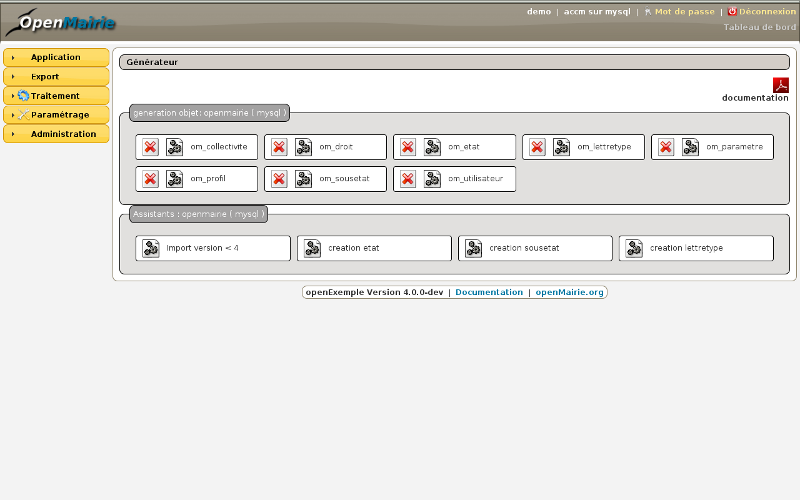
\includegraphics{ecran_1.png}

En appuyant sur la touche generation
on accède à l'écran de génération qui se décompose en :
\begin{itemize}
\item {} 
une analyse  de la base de donnée en cours et de la table choisie

\item {} 
un état des fichiers existants ou non

\item {} 
les options de génération

\end{itemize}

le choix du fichier de paramétrage par défaut

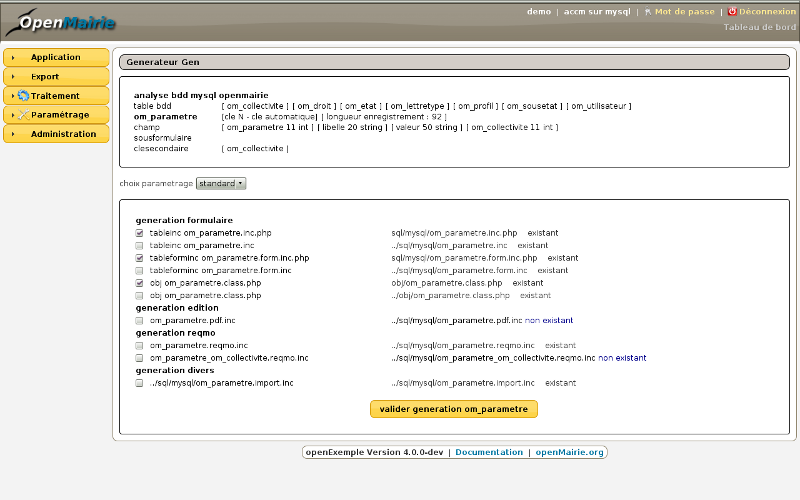
\includegraphics{ecran_2.png}


\subsubsection{Analyse de la base}

Le programme propose une analyse de la base en cours :
\begin{itemize}
\item {} 
liste des tables de la base

\item {} 
l'information sur la clé primaire de la table

\item {} 
la longueur de l'enregistrement de la table

\item {} 
les informations sur les champs : nom, type et longueur

\item {} 
les clés secondaires (exemple table om\_colllectivite

\item {} 
les sous formulaires à associer

\end{itemize}


\subsubsection{Les fichiers à generer}

Il est proposé une liste de case à cocher :

La case est cochée sur le fichier correspondant n'existe pas (colonne de droite)

Le formulaire métier auto généré, table.inc, tableform.inc est toujours coché (fichiers en gen/):
\begin{quote}

gen/obj/table.class.php

gen/sql/basededonnees/table.inc

sql/basededonnees/table.form.inc
\end{quote}

La génération de ces 3 fichiers ne met pas en péril votre programmation qui est en :
\begin{quote}

obj/table.class.php

sql/basededonnees/table.inc

sql/basededonnees/table.form.inc
\end{quote}

\resetcurrentobjects
\hypertarget{--doc-generateur/analyse_base}{}

\hypertarget{analyse-base}{}\subsection{L'analyse de la base}

Les informations de la base sont analysées par la méthode « constructeur » de gen.class.php

La construction des formulaires se fait suivant 4 types de champs reconnus par le générateur:

\begin{Verbatim}[commandchars=@\[\]]
- string : chaîne de caractère
- int : nombre (entier ou décimal)
- date
- blob : texte
\end{Verbatim}


\subsubsection{Type de champs}

la champ String est du type openMairie (méthode setType()):
\begin{itemize}
\item {} 
text dans le cas général

\item {} 
hiddenstatic si modification pour clé primaire

\item {} 
select pour clé secondaire

\end{itemize}

Le champ date est du type openMairie date avec calendrier et java script de contrôle de saisie de date

(La date est au format français JJ/MM/AAAA)

le champ Int est du type openMairie (methode setType())
\begin{itemize}
\item {} 
hidden si clé primaire en ajout

\item {} 
hiddenstatic si clé primaire en modification

\item {} 
text avec contrôle numérique en javascript

\item {} 
select pour clé secondaire

\end{itemize}

Le champ Blob est du type openMairie textarea

La longueur et la largeur sont définis en fichier de paramétrage form.inc

La taille n est pas pris en compte dans la longueur d'enregistrement

Les paramètres de dyn/form.inc permettent d'établir la longueur et la largeur d'affichage d'un blob :

\begin{Verbatim}[commandchars=@\[\]]
@$max=6; // nombre de ligne blob
    @$taille=80; // taille du blob
\end{Verbatim}


\subsubsection{Equivalence type mysql / type openMairie}

type mysql (longueur)          tableinfo   -\textgreater{} type openMairie

\begin{Verbatim}[commandchars=@\[\]]
Int         (taille mysql)                  -@textgreater[] Int
Date        (10)                            -@textgreater[] date
Blob        (65535)                         -@textgreater[] Blob
Char        (taille mysql)      char        -@textgreater[] String
tinyint     (4)                 tinyint     -@textgreater[] Int
smallint    (6)                 smallint    -@textgreater[] Int
Mediumint   (9)                 mediumint   -@textgreater[] Int
Bigint      (20)                bigint      -@textgreater[]Int
Float       (12)                Real        -@textgreater[] Int
Double      (22)                Real        -@textgreater[] Int
Decimal     (11)                Real        -@textgreater[] Int
Text        (65535)             Blob        -@textgreater[] Blob
Tinyblob    (255)               blob        -@textgreater[]Blob
Mediumblob  16777615            Blob        -@textgreater[] Blob
Mediumtext  16777215            Blob        -@textgreater[] Blob
Longtext    -1                  blob        -@textgreater[] Blob
Longblob    -1                  Blob        -@textgreater[] Blob
Tinytext    255                 Blob -      -@textgreater[] blob
\end{Verbatim}


\subsubsection{Equivalence type pgsql / type openMairie}

L'information fournie par postgresql est moins complète que celle de mysql surtout au niveau de la longueur des champs « string » où il est fourni :la longueur de stockage  qui est égal à -1 quand le stockage est variable

type pgsql (longueur) type tableinfo si different -\textgreater{} type openMairie

\begin{Verbatim}[commandchars=@\[\]]
Bigint      (8)                 int8        -@textgreater[] int
Smallint    (2)                 Int2        -@textgreater[] Int
Integer     (4)                 Int4        -@textgreater[] Int
Real        (4)                 Float4      -@textgreater[] Int
Doubleprecision (8)             Float8      -@textgreater[] Int
Numeric     (20)                Numeric     -@textgreater[] Int
Money       (8)                 Money       -@textgreater[] Int
Char        (1)                 Char        -@textgreater[] String   (Quelque soit la longueur= 1)
Character   (-1)                Bpchar      -@textgreater[] String (Utilisation de la longueur d'affichage)
Character varying (-1)          Varchar     -@textgreater[] String (Utilisation de la longueur d'affichage)
Text        (-1)                text        -@textgreater[] blob  (Utilisation des paramètres de form.inc)
Date        (4)                 Date        -@textgreater[] Date (Utilisation des paramètres de form.inc - @$pgsql@_longueur@_date)
\end{Verbatim}

Gestion des longueurs négatives :

Il est remonté dans l'analyse des informations de la base une valeur négative car le stockage dans postgresql est variable.
OpenMairie utilise alors la longueur d'affichage qui est donnée par la plus longue saisie dans un champ. Donc pour avoir la longueur exacte, il est conseillé de saisie un enregistrement avec les champs « string » saisie avec le nombre de caractères souhaités à l'affichage.

Dans le cas ou rien n'est saisi, il est proposé dans form.inc

\begin{Verbatim}[commandchars=@\[\]]
@$pgsql@_taille@_defaut = 20; // taille du champ par défaut si retour pg@_field@_prtlen =0
@$pgsql@_taille@_minimum = 10; // taille minimum d affichage d un champ
\end{Verbatim}


\subsubsection{Nom de champ et nom de table}

Attention au nom de tables ou de champs, évitez les termes SQL : match, table, index, type, len ... ou openMairie : objet pour les noms de champs ou table

Les règles suivantes sont spécifiques au générateur pour reconnaître
les clés primaires et les clés secondaires :

la cle primaire de la table a le même nom que la table

le cle secondaire a le même nom que la table fille

\resetcurrentobjects
\hypertarget{--doc-generateur/fichier_genere}{}

\hypertarget{fichier-genere}{}\subsection{Les fichiers générés}

Les fichiers générés concernent :
\begin{itemize}
\item {} 
les formulaires

\item {} 
les requêtes mémorisées

\item {} 
le script d'import de données

\end{itemize}


\subsubsection{Les formulaires}

Les formulaires sont génèrés suivant le nom de la table dans le répertoire sql, sous repertoire portant le nom de la base pour régler le problème de compatibilité SQL (concaténation, extraction ...)

Deux types de formulaire sont générés : type table, type form.


\paragraph{Paramétres de type table :}
\begin{itemize}
\item {} 
gen/sql/base/nom\_table.inc

\item {} 
sql/base/nom\_table.inc

\end{itemize}

Par défaut :
\begin{itemize}
\item {} 
tri en affichage vide

\item {} 
champ de recherche avec les champs string

\item {} 
pas d'affichage de champ blog

\item {} 
rattachement de sous formulaire

\item {} 
affichage de l'édition de la table

\end{itemize}

Dans le fichier paramètres : form.inc

\$serie = nombre d'enregistrement par page

\$ico = icône par defaut


\paragraph{Paramétres de type Form :}

gen/sql/base/nom\_table.form.inc

sql/base/nom\_table.form.inc

Dans le fichier paramètres : form.inc

\$ico = icône par defaut

Par défaut :
- tous les champs sont affichés les uns en dessous des autres


\subsubsection{Les Objets « métier »}

L'objet métier généré est stocké en gen/obj/nom\_table.class.php. Ce script ne doit pas être modifié car il est reconstitué à chaque génération :

Cela permet de pouvoir modifier la base de données (ajout, modification ou suppression de champs) et de regénérer tout ou partie de l'application

Un second script héritant de l'objet généré permet de surcharger les méthodes et de personnalisé l'objet métier.

Toutes les modifications doivent être faites dans ce script soit en héritant de la méthode,
soit en surchargeant la méthode.

L'objet à personnaliser est stocké en obj/nom\_table.class.php

Les méthodes  générés dans l'objet métier gen/obj/nom\_table.class.php sont par défaut les suivantes.

Le type de champs est :
\begin{quote}

. caché (hidden) en ajout pour la clé primaire automatique,

. modifiable en ajout si la clé primaire n'est pas automatique

. la clé primaire est visible sans possibilité de modifier en modification

. la clé secondaire n'est pas modifiable en sous formulaire si c'est la clé primaire du formulaire

. la clé secondaire est un champ select qui reprend les informations de la table liée

. la date est au format français
\end{quote}

La longueur d'affichage et le maximum autorisé à la saisie est celle contenu dans la base d'origine (retraitée pour les champs string de pgsql)

Le contrôle des clés secondaires des autres tables est généré : il n'est pas possible de supprimer un enregistrement si des enregistrements sont liés à la clé primaire

Les libellés sont les noms des champs.

Ce module sert pour le formulaire et le(s) sous formulaire(s).

Les méthodes qui peuvent être implémentés dans obj/nom\_table.class.php sont les suivantes
\begin{itemize}
\item {} 
verifier

\item {} 
regroupe et groupe pour modifier les présentations

\item {} 
trigger avant ou après l'enregistrement:

\item {} 
triggerajouter

\item {} 
triggermodifier

\item {} 
triggersupprimer

\item {} 
triggerajouterapres

\item {} 
triggermodifierapres

\item {} 
triggersupprimerapres

\end{itemize}

Les méthodes de l'objet généré en gen/obj  peuvent être surchargées totalement ou partiellement :

Exemple :
\begin{quote}

om\_profil.class.php :
\begin{quote}

surcharge des méthodes
\begin{quote}

setValFAjout setId,

verifierAjout

et setType car la clé primaire est numérique et non automatique
\end{quote}
\end{quote}

om\_utilisateur.class.php :
\begin{quote}

champ pwd pour mot de passe  methode partiellement surchargées (parent::setvalF(\$val);) setvalF, setType, setValsousformulare, surcharge avec un javascript de mise en majuscule du nom
\end{quote}
\end{quote}

Enfin, il est possible de mettre en place d'autres type de champs disponible dans openMairie
\begin{itemize}
\item {} 
ComboG  combo gauche
\begin{itemize}
\item {} 
comboD combo droit

\item {} 
Localisation (geolocalisation en x, y)

\item {} 
http (lien)

\item {} 
httpclick (lien)

\item {} 
Password (Mot de passe)

\item {} 
Pagehtml (Textearea pour affichage html)

\item {} 
Textdisabled (Text non modifiable)

\item {} 
Selectdisabled (Select non modifiable)

\item {} 
Textreadonly (Text non modifiable)

\item {} 
Hidden (champ caché)

\item {} 
Checkbox (case a cocher oui/non)

\item {} 
Upload (chargement d'un fichier)

\item {} 
voir (voir un fichier téléchargé)

\item {} 
Rvb (choisir une couleur rvn avec la Palette de couleur)

\end{itemize}

\end{itemize}


\subsubsection{Les états}

Seul l'état « pdf » est généré par le générateur

Dans le menu gen (generateur), les états sont générés automatiquement avec un assistant.

Cet assistant vous permet de construire un état :
\begin{itemize}
\item {} 
en choisissant une table de la base

\item {} 
en choisissant les champs à mettre dans l'état

\end{itemize}

L'etat est enregistré dans la table om\_etat et peut être modifié
menu-\textgreater{}administration -\textgreater{} etat

De la même manière, il est possible de créer un sous etat.

Il est possible de choisir le champ qui sera la clé secondaire en lien avec la table mère

Le sousetat est enregistré dans la table om\_sousetat et peut être modifié

menu-\textgreater{}administration -\textgreater{} sousetat

Le calcul de la largeur des colonnes est automatique dans les sous états et l'état pdf.

Attention :  les champs « blob » ne sont pas pris en compte dans les éditions.


\subsubsection{les requêtes mémorisées}

Les requêtes paramétrées sont crées suivant le principe suivant :
\begin{itemize}
\item {} 
une requête globale

\item {} 
une requête avec un champ select pour chaque clé secondaire (il est possible de sélectionner la requête à générer

\item {} 
Les autres champs sont sélectionnés à l'affichage

\end{itemize}

Les requêtes sont accessibles dans l'option du menu -\textgreater{} export.


\subsubsection{les imports}

Un script d'import des données est généré suivant le principe suivant :
\begin{itemize}
\item {} 
si la clé est automatique, génération du compteur

\item {} 
tous les champs sont importés

\item {} 
vérification de l'existence de la clé secondaire à chaque enregistrement

\end{itemize}

Les tables avec clés secondaires doivent donc être importées en dernier.

\resetcurrentobjects
\hypertarget{--doc-generateur/parametrage_generateur}{}

\hypertarget{parametrage-generateur}{}\subsection{Paramétrage générateur}

Le paramétrage de base est dans le répertoire gen/dyn/standard.
Il est possible de le modifier dans le répertoire custom ou dans un autre répertoire.
Le choix du paramétrage se fait à chaque génération.


\subsubsection{le paramétrage standard}

Le paramétrage standard est dans le répertoire gen/dyn/standard


\subsubsection{Form.inc}

Voici les paramètres pour la génération de formulaire

\begin{Verbatim}[commandchars=@\[\]]
@$serie = 15;                        nombre d'enregistrement par page'
@$ico ="../img/ico@_application.png"; icone DEPRECATED ?
@$max=6;                             nb de ligne blob
@$taille=80;                         taille du blob
@$pgsql@_taille@_defaut = 20;          taille du champ par defaut si retour pg@_field@_prtlen =0
@$pgsql@_taille@_minimum    = 10;      taille minimum d affichage d un champ
@$pgsql@_longueur@_date=12;            taille d'affichage de la date '
\end{Verbatim}


\subsubsection{Etat.inc}

Parametres

\begin{Verbatim}[commandchars=@\[\]]
@$variable='@&'; (indice precedent la variable)
// general
@$orientation='P';
@$format='A4';
// footer
@$footerfont='helvetica';
@$footerattribut='I';
@$footertaille='8';
// logo
@$logo='logopdf.png';
@$logoleft='58';
@$logotop='7';
// titre
@$titreleft='41';
@$titretop='36';
@$titrelargeur='130';
@$titrehauteur='10';
@$titrefont='helvetica';
@$titreattribut='B';
@$titretaille='15';
@$titrebordure='0';
@$titrealign='C';
// corps
@$corpsleft='7';
@$corpstop='57';
@$corpslargeur='195';
@$corpshauteur='5';
@$corpsfont='helvetica';
@$corpsattribut='';
@$corpstaille='10';
@$corpsbordure='0';
@$corpsalign='J';
// sous etat
@$se@_font='helvetica';
@$se@_margeleft='8';
@$se@_margetop='5';
@$se@_margeright='5';
@$se@_couleurtexte="array('0','0','0')";
\end{Verbatim}


\subsubsection{Sousetat.inc}

Parametres

\begin{Verbatim}[commandchars=@\[\]]
@$longueurtableau= 195;
@$variable='@&'; (indice precedent la variable)
//titre
@$titrehauteur=10;
@$titrefont='helvetica';
@$titreattribut='B';
@$titretaille=10;
@$titrebordure=0;
@$titrealign='L';
@$titrefond=0;
@$titrefondcouleur="array(255,255,255)";
@$titretextecouleur="array(0,0,0)";
// intervalle
@$intervalle@_debut=0;
@$intervalle@_fin=5;
// entete
@$entete@_flag=1;
@$entete@_fond=1;
@$entete@_orientation="array(0,0,0)";
@$entete@_hauteur=7;
@$entete@_fondcouleur="array(255,255,255)";
@$entete@_textecouleur="array(0,0,0)";
// tableau
@$tableau@_bordure=1;
@$tableau@_fontaille=10;
// bordure
@$bordure@_couleur="array(0,0,0)";
// sous etat fond
@$se@_fond1="array(243,246,246)";
@$se@_fond2="array(255,255,255)";
// cellule
@$cellule@_fond=1;
@$cellule@_hauteur=7;
// total
@$cellule@_fond@_total=1;
@$cellule@_fontaille@_total=10;
@$cellule@_hauteur@_total=15;
@$cellule@_fondcouleur@_total="array(255,255,255)";
// moyenne
@$cellule@_fond@_moyenne=1;
@$cellule@_fontaille@_moyenne=10;
@$cellule@_hauteur@_moyenne=5;
@$cellule@_fondcouleur@_moyenne="array(212,219,220)";
// nombre d enregistrement
@$cellule@_fond@_nbr=1;
@$cellule@_fontaille@_nbr=10;
@$cellule@_hauteur@_nbr=7;
@$cellule@_fondcouleur@_nbr="array(255,255,255)";
\end{Verbatim}


\subsubsection{Pdf.inc}

Parametres

\begin{Verbatim}[commandchars=@\[\]]
@$longueurtableau= 280;
@$orientation='L';// orientation P-@textgreater[] portrait L-@textgreater[]paysage";
@$format='A4';// format A3 A4 A5;
@$police='arial';
@$margeleft=10;// marge gauche;
@$margetop=5;// marge haut;
@$margeright=5;//  marge droite;
@$border=1; // 1 -@textgreater[]  bordure 0 -@textgreater[] pas de bordure";
@$C1=0;// couleur texte  R";
@$C2=0;// couleur texte  V";
@$C3=0;// couleur texte  B";
@$size=10; //taille POLICE";
@$height=4.6; // hauteur ligne tableau ";
@$align='L';
// fond 2 couleurs
@$fond=1;// 0- @textgreater[] FOND transparent 1 -@textgreater[] fond";
@$C1fond1=234;// couleur fond  R ";
@$C2fond1=240;// couleur fond  V ";
@$C3fond1=245;// couleur fond  B ";
@$C1fond2=255;// couleur fond  R";
@$C2fond2=255;// couleur fond  V";
@$C3fond2=255;// couleur fond  B";
// spe openelec
@$flagsessionliste=0;// 1 - @textgreater[] affichage session liste ou 0 -@textgreater[] pas d'affichage";
// titre
@$bordertitre=0; // 1 -@textgreater[]  bordure 0 -@textgreater[] pas de bordure";
@$aligntitre='L'; // L,C,R";
@$heightitre=10;// hauteur ligne titre";
@$grastitre='B';//\@$gras='B' -@textgreater[] BOLD OU \@$gras=''";
@$fondtitre=0; //0- @textgreater[] FOND transparent 1 -@textgreater[] fond";
@$C1titrefond=181;// couleur fond  R";
@$C2titrefond=182;// couleur fond  V";
@$C3titrefond=188;// couleur fond  B";
@$C1titre=75;// couleur texte  R";
@$C2titre=79;// couleur texte  V";
@$C3titre=81;// couleur texte  B";
@$sizetitre=15;
// entete colonne
@$flag@_entete=1;//entete colonne : 0 -@textgreater[] non affichage , 1 -@textgreater[] affichage";
@$fondentete=1;// 0- @textgreater[] FOND transparent 1 -@textgreater[] fond";
@$heightentete=10;//hauteur ligne entete colonne";
@$C1fondentete=210;// couleur fond  R";
@$C2fondentete=216;// couleur fond  V";
@$C3fondentete=249;// couleur fond  B";
@$C1entetetxt=0;// couleur texte R";
@$C2entetetxt=0;// couleur texte V";
@$C3entetetxt=0;// couleur texte B";
@$C1border=159;// couleur texte  R";
@$C2border=160;// couleur texte  V";
@$C3border=167;// couleur texte  B";
@$bt=1;// border 1ere  et derniere ligne  du tableau par page-@textgreater[]0 ou 1";
\end{Verbatim}


\subsubsection{Customiser le paramétrage}

Il est possible de personnaliser le paramétrage dans le répertoire custom ou en créant un autre répertoire avec des paramètres personnels.

Il faut mettre dans le répertoire le où les fichiers à personnaliser.

Ne personnaliser que les variables souhaitées dans le fichier. Par défaut, openMairie prendra les paramètres standards.

Choisir le paramétrage personnalisé dans l'écran de génération qui affiche les répertoires de paramètres existants.

Ne pas supprimer le répertoire  standard et les fichiers par défaut.


\chapter{Règles et outils}

\resetcurrentobjects
\hypertarget{--doc-regles/index}{}

\hypertarget{regles}{}\section{Les règles de codage}

La convention de codage openMairie s'applique à tout le code qui fait partie
de la distribution officielle d'openMairie. La convention de codage permet de
conserver un code consistant et de le rendre lisible et maintenable facilement
par les développeurs openMairie.

\resetcurrentobjects
\hypertarget{--doc-regles/indentation}{}

\hypertarget{indentation}{}\subsection{L'indentation du code}

Pour améliorer la lisibilité, il faut utiliser une indentation de 4 espaces et
non pas des tabulations. En effet, les éditeurs de texte interprètent
différemment les tabulations alors que les espaces sont tous interprétés de la
même façon. De plus lors de commit, les historiques des gestionnaires de
versions (CVS ou SVN) sont faussés par ces caractères.

Il est recommandé que la longueur des lignes ne dépasse pas 75 à 85 caractères.

\resetcurrentobjects
\hypertarget{--doc-regles/encodage}{}

\hypertarget{encodage}{}\subsection{L'encodage des fichiers}

Il vaut mieux mettre les accents dans les traductions plutôt que
de les intégrer dans les zones à traduire.

\emph{voir poedit}

\resetcurrentobjects
\hypertarget{--doc-regles/tags}{}

\hypertarget{tags}{}\subsection{Tags dans le code PHP}

Utilisez toujours \textless{}?php ?\textgreater{} pour délimiter du code PHP, et non la version
abrégée \textless{}? ?\textgreater{}. Cela est la méthode la plus portable pour inclure du code PHP
sur des systèmes d'exploitations disposant de configurations différentes.

\resetcurrentobjects
\hypertarget{--doc-regles/norme}{}

\hypertarget{norme}{}\subsection{Les normes à respecter}


\subsubsection{Pourquoi respecter des normes ?}

...


\subsubsection{XHTML Valide et le W3C}

...

\resetcurrentobjects
\hypertarget{--doc-regles/commentaire}{}

\hypertarget{commentaire}{}\subsection{Les commentaires dans le code}

Tous les fichiers PHP doivent avoir un entête de ce style

\begin{Verbatim}[commandchars=@\[\]]
@textless[]?php
/**
 * Courte description du fichier
 *
 * Description plus détaillée du fichier (si besoin en est)...
 *
 * @PYGZat[]package openmairie
 * @PYGZat[]version SVN : @$Id@$
 */

?@textgreater[]
\end{Verbatim}

\resetcurrentobjects
\hypertarget{--doc-regles/separation-contenu-presentation}{}

\hypertarget{separation-contenu-presentation}{}\subsection{Séparation du contenu et de la présentation dans le couple XHTML CSS}

...

\resetcurrentobjects
\hypertarget{--doc-regles/image}{}

\hypertarget{image}{}\subsection{Images}

Les fichiers images ajoutés dans les applications openMairie doivent être au
format PNG (Portable Network Graphics). Ce format permet d'obtenir des images
de qualité avec des propriétés de transparence.

\resetcurrentobjects
\hypertarget{--doc-versions/index}{}

\hypertarget{versions}{}\section{Le versionning du code et la version des applications}

\resetcurrentobjects
\hypertarget{--doc-versions/numerotation}{}

\hypertarget{numerotation}{}\subsection{Convention de numérotation des versions des applications et librairies}

Il est convenu de numéroter les versions sur 3 chiffres séparé par des points.

exemple: openMairie 4.0.0

Le premier chiffre représente une version majeure

Le deuxièeme chiffre est une évolution mineure

Le troisième chiffre est une correction de bug

Les versions beta sont indiqué en fin de numérotation et ne sont jamais maintenu.

Seule la dernière version opérationnelle est maintenu

\resetcurrentobjects
\hypertarget{--doc-versions/svn}{}

\hypertarget{svn}{}\subsection{Apache Subversion (SVN)}

\href{http://subversion.apache.org/}{Site officiel du projet SVN}


\subsubsection{Pré-requis}

Installer subversion :
\href{http://subversion.apache.org/packages.html}{http://subversion.apache.org/packages.html}


\subsubsection{L'arborescence}

Voici l'arborescence standard d'un projet versionné sur un SVN :

\begin{Verbatim}[commandchars=@\[\]]
/trunk/
/tags/
/branches/
\end{Verbatim}
\begin{itemize}
\item {} 
trunk/ : la version en cours de développement.

\item {} 
tags/ : les différentes versions publiées. Les dossiers dans tags/ sont des
copies du dossier trunk/ a un instant précis. Ils permettent de fixer une
version pour la publier. Il est interdit d'effectuer une modification dans un
de ces dossiers, la bonne méthode étant de faire la modification dans le
trunk/ et de faire une nouvelle version dans le dossier tags/.

\item {} 
branches/ : ...

\end{itemize}


\subsubsection{Les règles d'or}
\begin{itemize}
\item {} 
Ne jamais commiter dans un tag.

\item {} 
Ne jamais commiter sans message de commit.

\item {} 
Ne jamais tagger une version qui contient des externals vers un `trunk'.

\end{itemize}


\subsubsection{Les commandes basiques à connaître}

Récupérer une copie locale :

\begin{Verbatim}[commandchars=@\[\]]
svn co svn+ssh://nom-du-développeur@PYGZat[]scm.adullact.net/openmairie/openmairie@_exemple/trunk openmairie@_exemple
\end{Verbatim}

Mettre à jour sa copie locale :

\begin{Verbatim}[commandchars=@\[\]]
svn up
\end{Verbatim}

Voir l'état de sa copie locale :

\begin{Verbatim}[commandchars=@\[\]]
svn st
\end{Verbatim}

Voir la différence entre sa copie locale et le dépôt :

\begin{Verbatim}[commandchars=@\[\]]
svn diff
\end{Verbatim}

\begin{Verbatim}[commandchars=@\[\]]
svn ci
\end{Verbatim}


\subsubsection{Externals}

C'est une propriété sur le dépôt SVN permettant d'importer du code provenant
d'un dépôt différent.

Le fichier EXTERNALS.txt :

\begin{Verbatim}[commandchars=@\[\]]
@#
@# created by: svn propset svn:externals -F ./EXTERNALS.txt .
@#

openmairie svn://scm.adullact.net/svnroot/openmairie/openmairie/tags/4.0.0/
fpdf svn://scm.adullact.net/svnroot/openmairie/externals/fpdf/tags/1.6-min/
pear http://svn.php.net/repository/pear/pear-core/tags/PEAR-1.9.1/
db http://svn.php.net/repository/pear/packages/DB/tags/RELEASE@_1@_7@_13/
\end{Verbatim}

Appliquer les propriétés externals :

\begin{Verbatim}[commandchars=@\[\]]
svn propset svn:externals -F ./EXTERNALS.txt .
svn up
svn ci
\end{Verbatim}


\subsubsection{Keywords}


\subsubsection{Les clients graphiques}

Il est recommandé de savoir utiliser et d'utiliser subversion en ligne de
commande mais il existe quelques clients graphiques qui permettent de réaliser
certaines opérations d'une manière plus conviviale.
\begin{itemize}
\item {} 
Meld

\item {} 
TortoiseSVN

\item {} 
...

\end{itemize}


\subsubsection{Tutoriaux}


\paragraph{Importer un nouveau projet}

Un nouveau projet est une nouvelle application qui se base sur la dernière
version taggée d'openmairie\_exemple. Ce tutorial contient certains pré-requis
comme la création du projet sur la forge, le fait d'avoir un utilisateur avec
les droits corrects sur le projet, le fait d'avoir consulter la \href{https://adullact.net/scm/viewvc.php/openmairie\_exemple/tags/?root=openmairie}{dernière
version taggée d'openmairie\_exemple}

On se positionne dans la dossier tmp pour récupérer la dernière version
d'openmairie\_exemple

\begin{Verbatim}[commandchars=@\[\]]
cd /tmp
svn export --ignore-externals svn://scm.adullact.net/svnroot/openmairie/openmairie@_exemple/tags/@textless[]DERNIERE@_VERSION@_OPENMAIRIE@_EXEMPLE@textgreater[]/ openexemple
\end{Verbatim}

On cré l'arborescence standard sur le dépôt

\begin{Verbatim}[commandchars=@\[\]]
svn mkdir svn+ssh://@textless[]NOM@_DU@_DEVELOPPEUR@textgreater[]@PYGZat[]scm.adullact.net/svnroot/@textless[]NOUVEAU@_PROJET@textgreater[]/trunk
svn mkdir svn+ssh://@textless[]NOM@_DU@_DEVELOPPEUR@textgreater[]@PYGZat[]scm.adullact.net/svnroot/@textless[]NOUVEAU@_PROJET@textgreater[]/tags
svn mkdir svn+ssh://@textless[]NOM@_DU@_DEVELOPPEUR@textgreater[]@PYGZat[]scm.adullact.net/svnroot/@textless[]NOUVEAU@_PROJET@textgreater[]/branches
\end{Verbatim}

On se positionne dans le dossier précédemment importé pour importer sur le
dépôt son contenu

\begin{Verbatim}[commandchars=@\[\]]
cd openexemple
svn import . svn+ssh://@textless[]NOM@_DU@_DEVELOPPEUR@textgreater[]@PYGZat[]scm.adullact.net/svnroot/@textless[]NOUVEAU@_PROJET@textgreater[]/trunk
\end{Verbatim}

On se positionne dans son dossier de développement pour créer la copie
locale du projet

\begin{Verbatim}[commandchars=@\[\]]
cd @textasciitilde[]/public@_html/
svn co svn+ssh://@textless[]NOM@_DU@_DEVELOPPEUR@textgreater[]@PYGZat[]scm.adullact.net/svnroot/@textless[]NOUVEAU@_PROJET@textgreater[]/trunk @textless[]NOUVEAU@_PROJET@textgreater[]
\end{Verbatim}

On se positionne dans le dossier php de l'application pour appliquer
les externals

\begin{Verbatim}[commandchars=@\[\]]
cd @textless[]NOUVEAU@_PROJET@textgreater[]/php
svn propset svn:externals -F ./EXTERNALS.txt .
svn up
svn ci
\end{Verbatim}


\paragraph{Publier une nouvelle version}

Ce tutorial contient certains pré-requis comme le fait d'avoir un utilisateur
avec les droits corrects sur le projet ou connaître comment incrémenter le
numéro de version de l'application à publier.

Avant de publier une application, il faut vérifier que l'EXTERNALS de la
librairie openMairie ne pointe pas vers le `trunk'. Pour cela

\begin{Verbatim}[commandchars=@\[\]]
less php/EXTERNALS.txt

@#
@# created by: svn propset svn:externals -F ./EXTERNALS.txt .
@#

openmairie svn://scm.adullact.net/svnroot/openmairie/openmairie/trunk/
fpdf svn://scm.adullact.net/svnroot/openmairie/externals/fpdf/tags/1.6-min/
pear http://svn.php.net/repository/pear/pear-core/tags/PEAR-1.9.1/
db http://svn.php.net/repository/pear/packages/DB/tags/RELEASE@_1@_7@_13/
\end{Verbatim}

Ici on voit que openmairie pointe vers le `trunk'. Nous devons d'abord publier
la librairie

\begin{Verbatim}[commandchars=@\[\]]
svn cp svn+ssh://@textless[]NOM@_DU@_DEVELOPPEUR@textgreater[]@PYGZat[]scm.adullact.net/openmairie/openmairie/trunk svn+ssh://@textless[]NOM@_DU@_DEVELOPPEUR@textgreater[]@PYGZat[]scm.adullact.net/openmairie/openmairie/tags/@textless[]NOUVELLE@_VERSION@textgreater[]
\end{Verbatim}

Le message pourra être : Tag openmairie \textless{}NOUVELLE\_VERSION\textgreater{}.

Ensuite il faut changer les EXTERNALS.txt. On remplace dans le fichier
php/EXTERNALS.txt, le trunk par la nouvelle version

\begin{Verbatim}[commandchars=@\[\]]
vim php/EXTERNALS.txt

@#
@# created by: svn propset svn:externals -F ./EXTERNALS.txt .
@#

openmairie svn://scm.adullact.net/svnroot/openmairie/openmairie/tags/@textless[]NOUVELLE@_VERSION@textgreater[]/
fpdf svn://scm.adullact.net/svnroot/openmairie/externals/fpdf/tags/1.6-min/
pear http://svn.php.net/repository/pear/pear-core/tags/PEAR-1.9.1/
db http://svn.php.net/repository/pear/packages/DB/tags/RELEASE@_1@_7@_13/
\end{Verbatim}

Ensuite on applique le nouveau propset externals une fois placé dans le dossier
php (Attention de ne pas oublier le ``.'' dans la commande svn propset)

\begin{Verbatim}[commandchars=@\[\]]
cd php/
svn propset svn:externals -F ./EXTERNALS.txt .
svn up
\end{Verbatim}

Ici en faisant un svn info sur le dossier openmairie, nous devons obtenir une
URL comme ceci

\begin{Verbatim}[commandchars=@\[\]]
svn info openmairie/
URL : svn://scm.adullact.net/svnroot/openmairie/openmairie/tags/@textless[]NOUVELLE@_VERSION@textgreater[]
\end{Verbatim}

Si tout est ok nous pouvons valider nos modifications puis passer à la
publication de l'application

\begin{Verbatim}[commandchars=@\[\]]
svn ci
\end{Verbatim}

Ici on fait une copie du `trunk' vers le dossier `tags' de l'application
openmairie\_exemple

\begin{Verbatim}[commandchars=@\[\]]
svn cp svn+ssh://@textless[]NOM@_DU@_DEVELOPPEUR@textgreater[]@PYGZat[]scm.adullact.net/openmairie/openmairie@_exemple/trunk svn+ssh://@textless[]NOM@_DU@_DEVELOPPEUR@textgreater[]@PYGZat[]scm.adullact.net/openmairie/openmairie@_exemple/tags/@textless[]NOUVELLE@_VERSION@textgreater[]
\end{Verbatim}

\resetcurrentobjects
\hypertarget{--doc-versions/cvs}{}

\hypertarget{cvs}{}\subsection{Concurrent versions system (CVS)}

\href{http://www.nongnu.org/cvs/}{Site officiel du projet CVS}

\resetcurrentobjects
\hypertarget{--doc-outils/index}{}

\hypertarget{outils}{}\section{Les outils du développeur}

Les sites de référence :
\begin{itemize}
\item {} 
\href{http://php.net/}{http://php.net/}

\end{itemize}

Les outils indispensables :

\resetcurrentobjects
\hypertarget{--doc-outils/firefox}{}

\hypertarget{firefox}{}\subsection{Le navigateur Mozilla Firefox}

\href{http://www.mozilla-europe.org/fr/firefox/}{Mozilla Firefox}

Ses modules complémentaires indispensables au développement Web :


\subsubsection{Web Developer}

\href{https://addons.mozilla.org/fr/firefox/addon/60/}{Web Developer}


\subsubsection{Firebug}

\href{https://addons.mozilla.org/fr/firefox/addon/1843/}{Firebug}


\subsubsection{HTML Validator}

\href{https://addons.mozilla.org/fr/firefox/addon/249/}{HTML Validator}


\subsubsection{YSlow}

\href{https://addons.mozilla.org/fr/firefox/addon/5369/}{YSlow}

\resetcurrentobjects
\hypertarget{--doc-outils/komodo-edit}{}

\hypertarget{komodo-edit}{}\subsection{Komodo Edit}

Free Code Editor for Windows, Mac and Linux

\href{http://www.activestate.com/komodo-edit}{http://www.activestate.com/komodo-edit}

\href{http://www.activestate.com/komodo-edit/downloads}{http://www.activestate.com/komodo-edit/downloads}

\resetcurrentobjects
\hypertarget{--doc-outils/meld}{}

\hypertarget{meld}{}\subsection{Meld}

\resetcurrentobjects
\hypertarget{--doc-outils/poedit}{}

\hypertarget{poedit}{}\subsection{POEdit}

...
\begin{itemize}
\item {} 
TortoiseSVN

\item {} 
TortoiseCVS

\end{itemize}

L'environnement de développement :
\begin{itemize}
\item {} 
Apache

\item {} 
PHP

\item {} 
EasyPHP

\item {} 
Wamp

\item {} 
Lamp

\end{itemize}


\chapter{Contributeurs}
\begin{itemize}
\item {} 
\href{mailto:fmichon@atreal.net}{Florent Michon {[}ATREAL{]}}

\item {} 
\href{mailto:contact@openmairie.org}{Francois Raynaud}

\end{itemize}


\renewcommand{\indexname}{Index du module}
\printmodindex
\renewcommand{\indexname}{Index}
\printindex
\end{document}
